% Options for packages loaded elsewhere
\PassOptionsToPackage{unicode}{hyperref}
\PassOptionsToPackage{hyphens}{url}
%
\documentclass[
  a4paper,
]{scrbook}

\usepackage{amsmath,amssymb}
\usepackage{iftex}
\ifPDFTeX
  \usepackage[T1]{fontenc}
  \usepackage[utf8]{inputenc}
  \usepackage{textcomp} % provide euro and other symbols
\else % if luatex or xetex
  \usepackage{unicode-math}
  \defaultfontfeatures{Scale=MatchLowercase}
  \defaultfontfeatures[\rmfamily]{Ligatures=TeX,Scale=1}
\fi
\usepackage{lmodern}
\ifPDFTeX\else  
    % xetex/luatex font selection
  \setmainfont[]{Latin Modern Roman}
  \setsansfont[]{Latin Modern Roman}
\fi
% Use upquote if available, for straight quotes in verbatim environments
\IfFileExists{upquote.sty}{\usepackage{upquote}}{}
\IfFileExists{microtype.sty}{% use microtype if available
  \usepackage[]{microtype}
  \UseMicrotypeSet[protrusion]{basicmath} % disable protrusion for tt fonts
}{}
\makeatletter
\@ifundefined{KOMAClassName}{% if non-KOMA class
  \IfFileExists{parskip.sty}{%
    \usepackage{parskip}
  }{% else
    \setlength{\parindent}{0pt}
    \setlength{\parskip}{6pt plus 2pt minus 1pt}}
}{% if KOMA class
  \KOMAoptions{parskip=half}}
\makeatother
\usepackage{xcolor}
\setlength{\emergencystretch}{3em} % prevent overfull lines
\setcounter{secnumdepth}{5}
% Make \paragraph and \subparagraph free-standing
\ifx\paragraph\undefined\else
  \let\oldparagraph\paragraph
  \renewcommand{\paragraph}[1]{\oldparagraph{#1}\mbox{}}
\fi
\ifx\subparagraph\undefined\else
  \let\oldsubparagraph\subparagraph
  \renewcommand{\subparagraph}[1]{\oldsubparagraph{#1}\mbox{}}
\fi


\providecommand{\tightlist}{%
  \setlength{\itemsep}{0pt}\setlength{\parskip}{0pt}}\usepackage{longtable,booktabs,array}
\usepackage{calc} % for calculating minipage widths
% Correct order of tables after \paragraph or \subparagraph
\usepackage{etoolbox}
\makeatletter
\patchcmd\longtable{\par}{\if@noskipsec\mbox{}\fi\par}{}{}
\makeatother
% Allow footnotes in longtable head/foot
\IfFileExists{footnotehyper.sty}{\usepackage{footnotehyper}}{\usepackage{footnote}}
\makesavenoteenv{longtable}
\usepackage{graphicx}
\makeatletter
\def\maxwidth{\ifdim\Gin@nat@width>\linewidth\linewidth\else\Gin@nat@width\fi}
\def\maxheight{\ifdim\Gin@nat@height>\textheight\textheight\else\Gin@nat@height\fi}
\makeatother
% Scale images if necessary, so that they will not overflow the page
% margins by default, and it is still possible to overwrite the defaults
% using explicit options in \includegraphics[width, height, ...]{}
\setkeys{Gin}{width=\maxwidth,height=\maxheight,keepaspectratio}
% Set default figure placement to htbp
\makeatletter
\def\fps@figure{htbp}
\makeatother

\usepackage{booktabs}
\usepackage{longtable}
\usepackage{array}
\usepackage{multirow}
\usepackage{wrapfig}
\usepackage{float}
\usepackage{colortbl}
\usepackage{pdflscape}
\usepackage{tabu}
\usepackage{threeparttable}
\usepackage{threeparttablex}
\usepackage[normalem]{ulem}
\usepackage{makecell}
\usepackage{xcolor}
\usepackage{titling}
\setlength{\droptitle}{-2cm}
\preauthor{
  \begin{center}
  \Large
  \vspace{10mm}
  by

  \vspace{20mm}
}
\postauthor{
  \end{center}
  \vfill
}

\predate{
  \begin{center}
  A thesis 
  submitted in fulfilment of the \\
  requirements of the degree of \\
  Doctor of Philosophy in Physics\\               % Degree
  School of Physical and Chemical Sciences\\          % Department
  Te Herenga Waka - Victoria University of Wellington\\                       % University 
  \vspace{5mm}
}
\postdate{
  \\
  
\includegraphics[width=3in,height=1.5in]{figures/VUW-logo.png}\\
  \end{center}
  }
\makeatletter
\makeatother
\makeatletter
\@ifpackageloaded{bookmark}{}{\usepackage{bookmark}}
\makeatother
\makeatletter
\@ifpackageloaded{caption}{}{\usepackage{caption}}
\AtBeginDocument{%
\ifdefined\contentsname
  \renewcommand*\contentsname{Table of contents}
\else
  \newcommand\contentsname{Table of contents}
\fi
\ifdefined\listfigurename
  \renewcommand*\listfigurename{List of Figures}
\else
  \newcommand\listfigurename{List of Figures}
\fi
\ifdefined\listtablename
  \renewcommand*\listtablename{List of Tables}
\else
  \newcommand\listtablename{List of Tables}
\fi
\ifdefined\figurename
  \renewcommand*\figurename{Figure}
\else
  \newcommand\figurename{Figure}
\fi
\ifdefined\tablename
  \renewcommand*\tablename{Table}
\else
  \newcommand\tablename{Table}
\fi
}
\@ifpackageloaded{float}{}{\usepackage{float}}
\floatstyle{ruled}
\@ifundefined{c@chapter}{\newfloat{codelisting}{h}{lop}}{\newfloat{codelisting}{h}{lop}[chapter]}
\floatname{codelisting}{Listing}
\newcommand*\listoflistings{\listof{codelisting}{List of Listings}}
\makeatother
\makeatletter
\@ifpackageloaded{caption}{}{\usepackage{caption}}
\@ifpackageloaded{subcaption}{}{\usepackage{subcaption}}
\makeatother
\makeatletter
\@ifpackageloaded{tcolorbox}{}{\usepackage[skins,breakable]{tcolorbox}}
\makeatother
\makeatletter
\@ifundefined{shadecolor}{\definecolor{shadecolor}{rgb}{.97, .97, .97}}
\makeatother
\makeatletter
\makeatother
\makeatletter
\makeatother
\ifLuaTeX
  \usepackage{selnolig}  % disable illegal ligatures
\fi
\usepackage[citestyle = ieee,urldate = iso8601]{biblatex}
\addbibresource{references.bib}
\IfFileExists{bookmark.sty}{\usepackage{bookmark}}{\usepackage{hyperref}}
\IfFileExists{xurl.sty}{\usepackage{xurl}}{} % add URL line breaks if available
\urlstyle{same} % disable monospaced font for URLs
\hypersetup{
  pdftitle={Volatile Organic Compound Detection Using Insect Odorant-Receptor Functionalised Field-Effect Transistors},
  pdfauthor={Eddyn Oswald Perkins Treacher},
  hidelinks,
  pdfcreator={LaTeX via pandoc}}

\title{Volatile Organic Compound Detection Using Insect Odorant-Receptor
Functionalised Field-Effect Transistors}
\author{Eddyn Oswald Perkins Treacher}
\date{May 2024}

\begin{document}
\frontmatter
\maketitle
\ifdefined\Shaded\renewenvironment{Shaded}{\begin{tcolorbox}[sharp corners, breakable, borderline west={3pt}{0pt}{shadecolor}, interior hidden, frame hidden, enhanced, boxrule=0pt]}{\end{tcolorbox}}\fi

\renewcommand*\contentsname{Table of contents}
{
\setcounter{tocdepth}{2}
\tableofcontents
}
\mainmatter
\bookmarksetup{startatroot}

\hypertarget{acknowledgements}{%
\chapter*{Acknowledgements}\label{acknowledgements}}
\addcontentsline{toc}{chapter}{Acknowledgements}

\markboth{Acknowledgements}{Acknowledgements}

\begin{verbatim}
69450
\end{verbatim}

Rifat, Alex - vapour sensor Erica Cassie - FET sensing setup Rob Keyzers
and Jennie Ramirez-Garcia - NMR spectra Patricia Hunt - Computational
chemistry

\bookmarksetup{startatroot}

\hypertarget{carbon-nanotube-and-graphene-field-effect-transistors}{%
\chapter{Carbon Nanotube and Graphene Field-Effect
Transistors}\label{carbon-nanotube-and-graphene-field-effect-transistors}}

\hypertarget{introduction}{%
\section{Introduction}\label{introduction}}

Out of a wide range of available transducer options available for the
creation of compact, portable and highly-integrated biosensors,
field-effect transistors are among the most promising. Field-effect
transistors consist of two conductive electrodes on either side of a
semiconducting channel, the `source' and `drain' electrodes, alongside
an isolated `gate' electrode. An applied electric field from the gate
electrode capacitively controls channel resistance, giving rise to the
label `field-effect'. By adjusting gate voltage, the flow of charge
carriers between source and drain can be varied over several orders of
magnitude. The ability of this simple structure to obtain a large signal
response from small changes in channel behaviour means field-effect
transistors can be used as high-quality amplifiers for sensor
applications \autocite{Shkodra2021,Yao2021}. Field-effect transistors
are typically unipolar transistors; channel conduction either mainly
consists of electron carriers, or hole carriers, depending on the
electrode and channel materials used \autocite{Yao2021}.

Carbon nanotube network and graphene field-effect transistors (CNTFETs
and GFETs) are both examples of a class of field-effect transistors
called thin-film transistors (TFTs). These transistors are closely
related to the commonly-used metal oxide semiconductor field-effect
transistor (MOSFET). Unlike MOSFETs, thin-film transistors do not use
the substrate as the device channel. Instead, current passes through a
semiconducting film on the surface of the device. Since thin-film
transistors do not require a conductive substrate, they can be
fabricated using flexible and stretchable substrates, and so are
significantly more versatile than MOSFETs. A wide variety of
semiconducting films may be used; the films discussed here are carbon
nanotube networks and graphene, which both fall under the class of
carbon-based 2D nanomaterials. Commonly used substrates include
silicon/silicon dioxide, quartz, glass, and the flexible substrates
polyimide (PI) and polyethylene terephthalate (PET)
\autocite{Sun2013,Shkodra2021}.

\hypertarget{sec-general-FETs}{%
\section{Thin-Film Field-Effect Transistors}\label{sec-general-FETs}}

\hypertarget{sec-gating}{%
\subsection{Structure and Gating}\label{sec-gating}}

The basic components of the thin-film transistor can be configured in a
variety of different ways. These configurations include the back-gated
field-effect transistor and the liquid-gated transistor, also known as
the electrolyte-gated transistor. The relatively simple back-gated
configuration, shown in Figure~\ref{fig-gating-schematics} (a), uses the
silicon substrate as the gate. The channel is isolated from the gate
with a thin silicon dioxide layer. A liquid-gated device, shown in
Figure~\ref{fig-gating-schematics} (b), is used for sensitive liquid
analyte detection. In the most common form of this configuration, a
Ag/AgCl reference electrode is used as the gate. The channel is isolated
from the gate by the bulk of an electrolyte solution, typically the
biofriendly phosphate-buffered saline (PBS). Other aqueous salt
solutions, polymers and ion-gels are also sometimes used as the
electrolyte gate. The electrolyte is restricted to the channel area
using a hydrophobic PDMS microchamber, referred to here as a `PDMS well'
\autocite{Avouris2007,Shkodra2021,Li2023}.

\begin{figure}

\begin{minipage}[t]{0.03\linewidth}

{\centering 

\raisebox{-\height}{

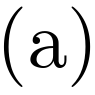
\includegraphics{figures/(a).png}

}

}

\end{minipage}%
%
\begin{minipage}[t]{0.01\linewidth}

{\centering 

~

}

\end{minipage}%
%
\begin{minipage}[t]{0.45\linewidth}

{\centering 

\raisebox{-\height}{

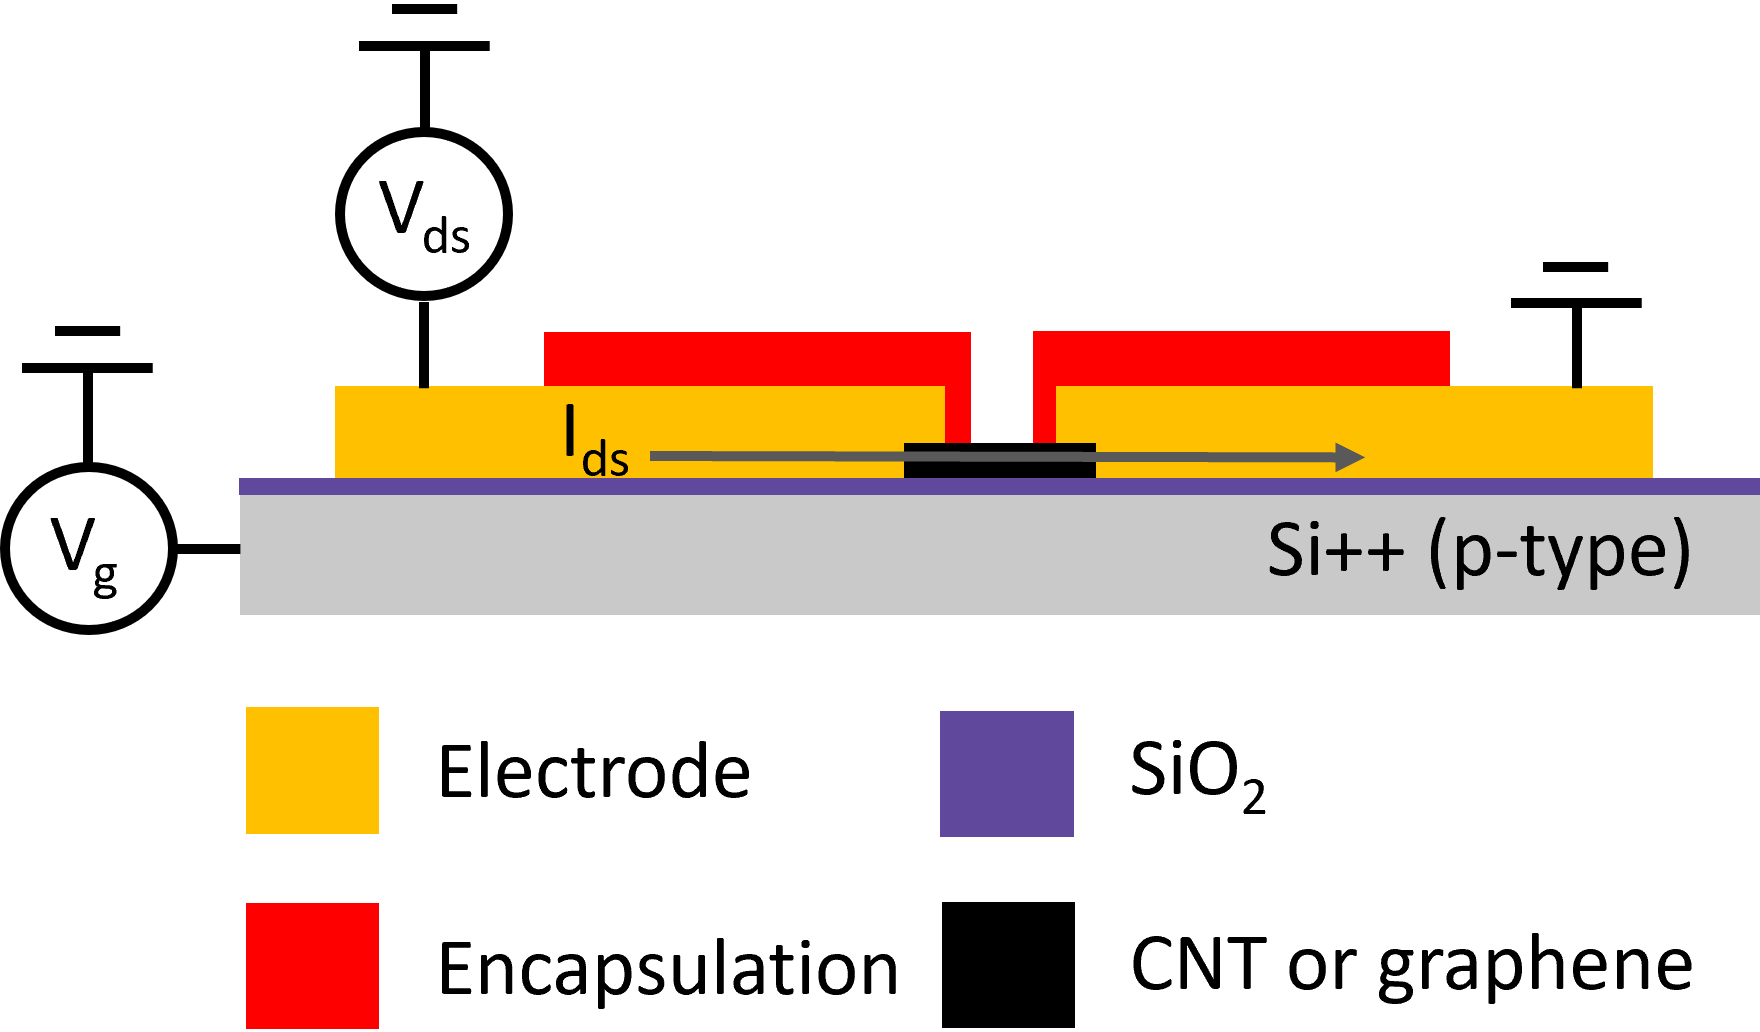
\includegraphics{figures/ch2/back-gate-schematic.png}

}

}

\end{minipage}%
%
\begin{minipage}[t]{0.01\linewidth}

{\centering 

~

}

\end{minipage}%
%
\begin{minipage}[t]{0.03\linewidth}

{\centering 

\raisebox{-\height}{

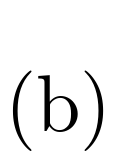
\includegraphics{figures/(b).png}

}

}

\end{minipage}%
%
\begin{minipage}[t]{0.01\linewidth}

{\centering 

~

}

\end{minipage}%
%
\begin{minipage}[t]{0.45\linewidth}

{\centering 

\raisebox{-\height}{

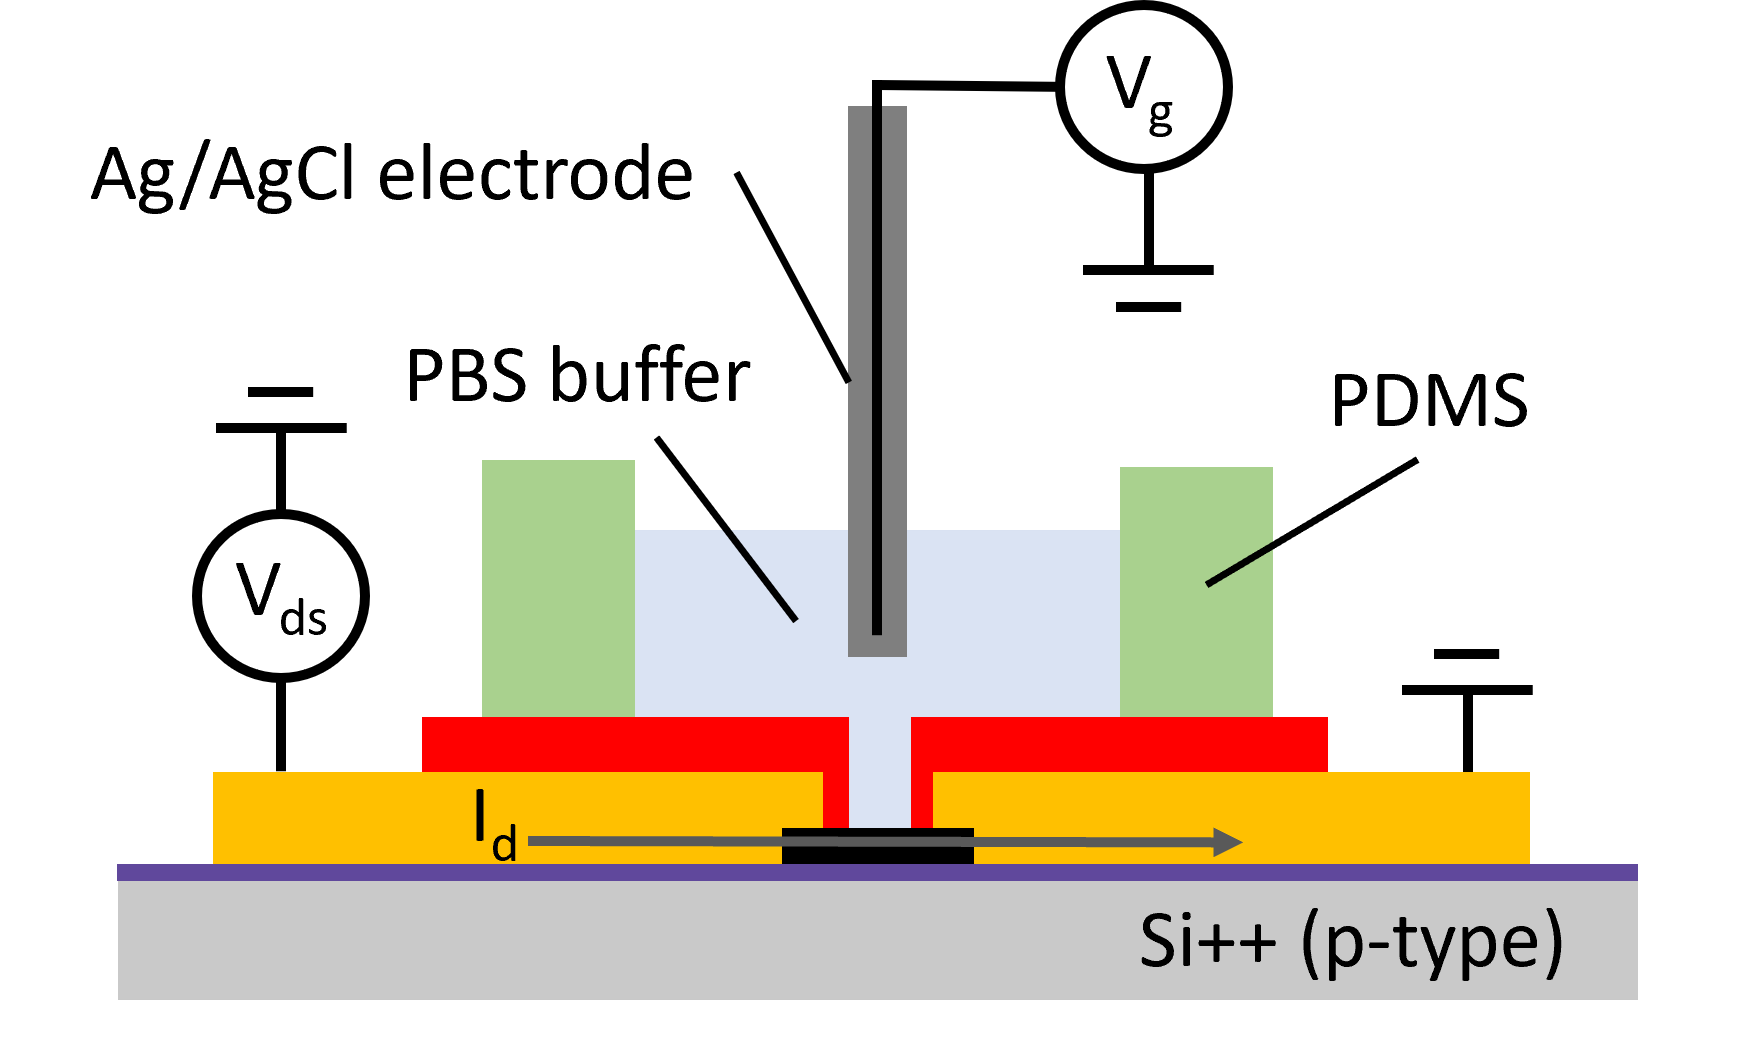
\includegraphics{figures/ch2/liquid-gate-schematic.png}

}

}

\end{minipage}%
%
\begin{minipage}[t]{0.01\linewidth}

{\centering 

~

}

\end{minipage}%

\caption{\label{fig-gating-schematics}Schematics (not to scale) showing
the side-view cross-section of a thin-film field-effect transistor in
both the (a) back-gated and (b) liquid-gated configuration. A graphene
monolayer or a carbon nanotube network is used as the transistor
thin-film. The drain electrode is the gold contact on the left side of
each figure, while the source electrode is the gold contact on the
right.}

\end{figure}

When the source and drain electrodes of a thin-film field-effect
transistor are made of metal, a Schottky barrier forms between the
channel and the electrodes. The Schottky barrier results from a
difference in the work function between the metal and semiconducting
channel, leading to bending of the conduction and valence bands and the
formation of an electric dipole layer at the junction. Due to the
absence of metal-channel bonding, the metal used has a direct impact on
barrier height \(\phi_B\) \autocite{Avouris2007,Li2023}. The spatial
extent of the dipole layer is called the barrier thickness. For unipolar
transistors, where the Schottky barrier is thick, the channel-electrode
contact determines the type of charge carrier passing between source and
drain. A contact which forms a low Schottky barrier for holes will form
a high Schottky barrier for electrons. In this case, holes flow and the
device is \(p\)-type. The reverse applies for a contact with a high
Schottky barrier for holes, where electrons flow and the device is
\(n\)-type. Thin-film devices can also be ambipolar, where charge
carriers can quantum-mechanically tunnel through thin Schottky barriers
and electrons and holes can both flow through the channel
\autocite{Avouris2007,Heller2008,Shkodra2021,Yao2021}.

Two different voltages are used to adjust transistor operation. The
first is the `drain bias', \(V_{ds}\), between the drain and source
electrodes, and the second is the `gate bias', \(V_g\), applied between
the gate and source electrode. Changing \(V_g\) alters the energy band
bending at the channel-electrode junctions, and therefore also alters
the energy barriers at these junctions. The value of \(V_g\) therefore
determines whether charge carriers may flow under the influence of
\(V_{ds}\) and produce a drain-source current \(I_d\); in other words,
\(V_g\) determines whether the transistor is `on' or `off'. The
threshold voltage \(V_t\) is the gate voltage required to increase the
Schottky barrier height to a point where charge carriers no longer flow.
For a \(p\)-type semiconductor channel, increasing \(V_g\) towards
positive gate voltages will raise the Schottky barrier and turn current
off, with the opposite being true for an \(n\)-type channel. In an
ambipolar transistor, a highly negative \(V_g\) will give rise to hole
conduction, and a highly positive \(V_g\) will give rise to electron
conduction. There are therefore two threshold voltages for these
devices, \(V_{t,h}\) and \(V_{t,e}\). Within the range between these
gate voltages, both holes and electrons flow through the channel
\autocite{Avouris2007,Reiner-Rozman2015,Yao2021,Li2023}.

The type of structure used determines the type of biological sensing
mechanisms available, which can include electrostatic gating, Schottky
barrier modulation, capacitance modulation or charge scattering.
Response mechanisms may take place at the gate, at the junctions between
channel and contact, or within the semiconductor channel
\autocite{Heller2008,Li2023}. The encapsulation layer shown in
Figure~\ref{fig-gating-schematics} is added to separate the electrodes
from the channel-metal junction, ensuring that the less-reliable
response due to modification of the channel-metal Schottky barrier does
not dominate sensing \autocite{Heller2008,Yao2021}. Encapsulation is
therefore a vital part of a functioning sensor, despite being
under-examined in the literature \autocite{Shkodra2021}. In an
encapsulated device with a semiconducting thin-film, the predominant
sensing mechanism is electrostatic gating. Here, the presence of a
positive charge induces negative charge in the channel or \emph{vice
versa}, in effect doping the channel and altering the relationship
between \(V_g\) and \(I_d\) \autocite{Heller2008}. The relative effect
of changes in \(V_g\) on \(I_d\) is determined by gate capacitance,
which is a series combination of the geometric capacitance, \(C_{G}\),
and the quantum capacitance of the 2D nanomaterial, \(C_{Q}\). For a
back-gated device, geometric capacitance is predominantly due to the
oxide layer capacitance \(C_{ox}\) \autocite{Heller2009a,Li2023}.

\hypertarget{liquid-gating-and-debye-length}{%
\subsubsection*{Liquid-Gating and Debye
Length}\label{liquid-gating-and-debye-length}}
\addcontentsline{toc}{subsubsection}{Liquid-Gating and Debye Length}

\begin{figure}

{\centering 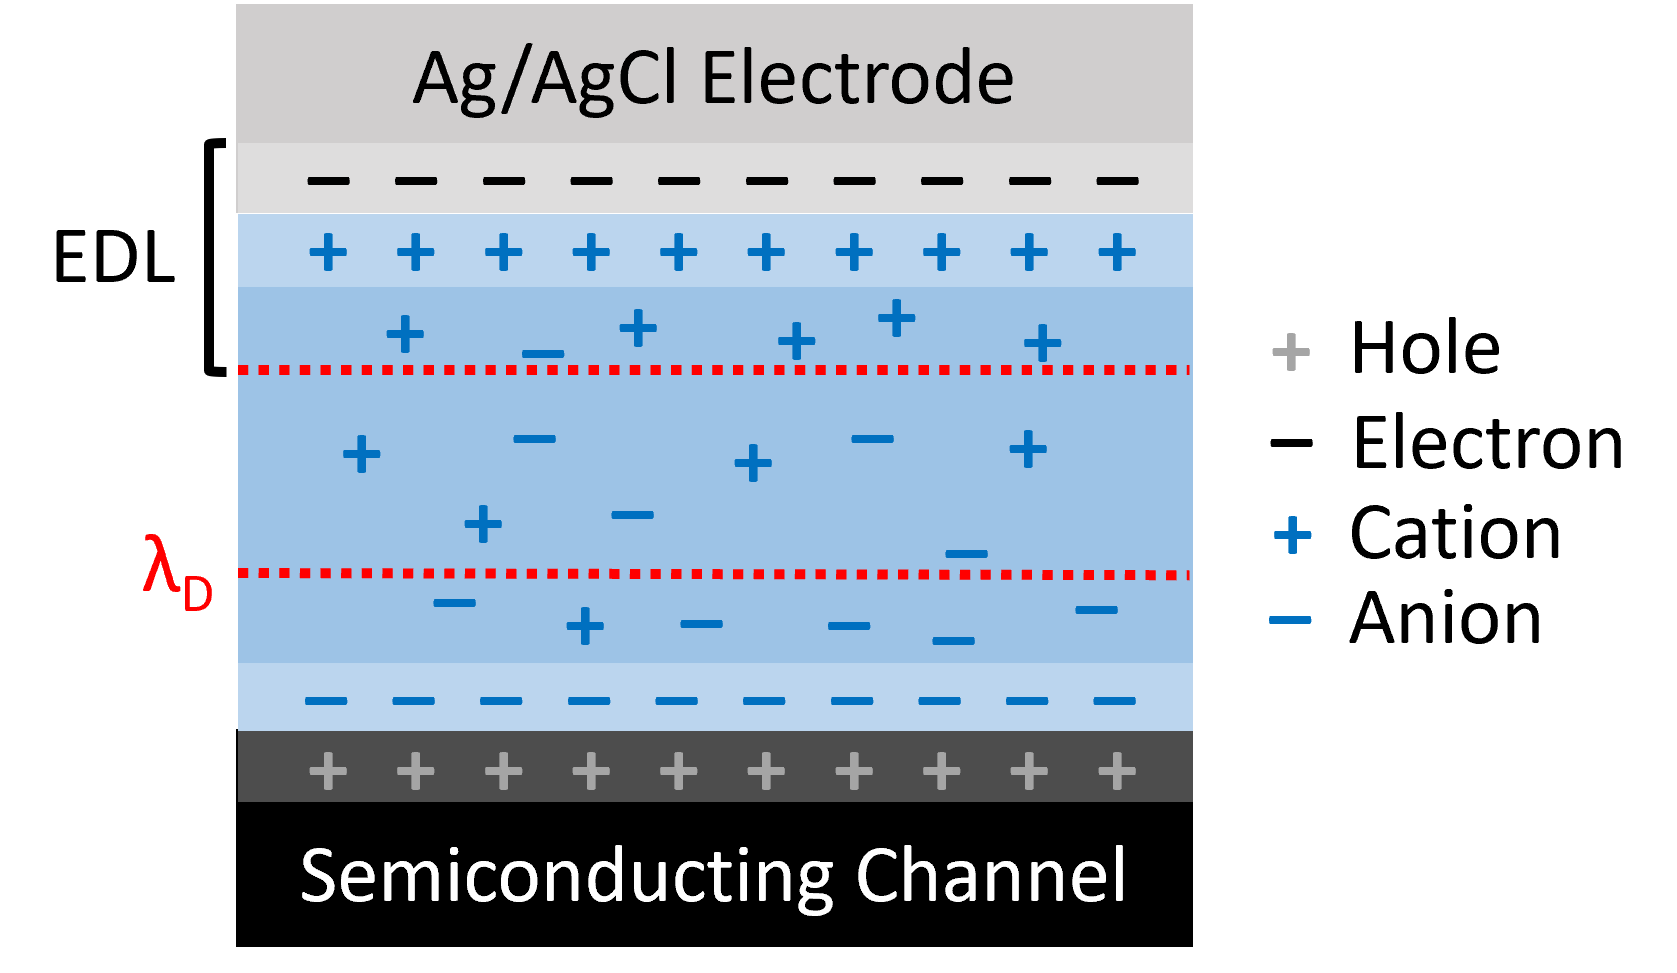
\includegraphics[width=0.7\textwidth,height=\textheight]{figures/ch2/Debye-length-schematic.png}

}

\caption{\label{fig-Debye-length}A diagram of the formation of an
electric double layer (EDL) under an applied voltage between source and
liquid-gate electrodes, with a \(p\)-type semiconductor used for the
channel thin-film. Electric double layers are present at both the
gate-electrolyte interface and semiconductor-electrolyte interface.
Adapted from \autocite{Shkodra2021,Tiwari2022}}

\end{figure}

Understanding the ionic behaviour of the gate electrolyte used in a
liquid-gated device setup gives insight into the gating and sensing
behaviour of the setup. When a voltage is applied at the liquid-gate,
the charged ions in solution move to form two electric double layers,
one at the interface between the electrolyte and gate electrode, and one
at the interface between electrolyte and semiconducting channel, as
shown in Figure~\ref{fig-Debye-length}. The gate capacitance is a series
combination of the capacitance of each EDL in series with quantum
capacitance \(C_{Q}\). The Gouy-Chapman-Stern model splits the EDL into
two distinct regions, the first being a compact layer of ions, the Stern
layer, and the second being a more diffuse layer, the Gouy-Chapman
layer. The surface potential of the solid-electrolyte interface
exponentially decreases across the diffuse region of the double-layer;
the characteristic length of this potential screening is known as Debye
length, \(\lambda_D\). The typical electrolyte Debye length is on a
nanometer scale, therefore the bulk electrolyte acts as an insulator,
similar to the silicon dioxide dielectric in the back-gated
configuration. The Stern layer capacitance is inversely proportional to
the Debye length, and therefore decreased \(\lambda_D\) corresponds to
increased gate capacitance
\autocite{Bard2001,Israelachvili2011,Shkodra2021,Tiwari2022}.

\begin{equation}\protect\hypertarget{eq-debye-length}{}{
\lambda_D = \sqrt{\frac{\epsilon_0\epsilon_rk_bT}{2N_Aq^2I}}
}\label{eq-debye-length}\end{equation}

The equation for Debye length \(\lambda_D\) in an electrolyte solution
is given by Equation~\ref{eq-debye-length}, where \(\epsilon_0\) is
vacuum permittivity, \(\epsilon_r\) is the relative permittivity of the
electrolyte, \(\k_B\) is the Boltzmann constant, \(T\) is absolute
temperature in K, \(N_A\) is the Avogadro number, \(q\) is the
elementary charge and \(I\) is ionic strength in mmol L\(^{-1}\). When
temperature is kept constant, \(\lambda_D\) only depends on the ionic
strength of the electrolyte and not on any attributes of the gate
electrode or channel. Successive dilutions of a particular electrolyte
will increase the Debye length: for \(1 \times\) PBS, \(\lambda_D\) is
0.7 nm, for \(0.1 \times\) PBS, \(\lambda_D\) is 2.3 nm, for
\(0.01 \times\) PBS \(\lambda_D\) is 7.3 nm and so on. This means gate
capacitance is directly dependent on the electrolyte used and its
concentration. A \(1 \times\) PBS electrolyte gives a gate capacitance
several orders of magnitude larger than that of a silicon oxide
back-gate, where a larger capacitance significantly increases the effect
of electrostatic gating on the channel current. A liquid-gated device
with low Debye length will therefore be highly sensitive to
electrostatic changes across a small voltage range
\autocite{Israelachvili2011,Shkodra2021}.

However, a decreased Debye length also has disadvantages for sensing.
Electrostatic potentials outside of the electrolyte-channel electrical
double layer are effectively screened from the channel. Electrical
double layers will also form around biomolecules such as DNA present
within the solution. The combined screening effect means signals due to
potential changes in charged biomolecules within the bulk electrolyte
will have no effect on gating of the channel. Interactions between the
analyte and any biorecognition element must therefore occur within the
Debye length. A tradeoff has to be made between channel sensitivity and
the size of the sensitive region above the channel. Many medium or large
proteins will require a relatively dilute electrolyte for analyte
capture to be detected by the channel
\autocite{Stern2007,Piccinini2018,Shkodra2021}. Other approaches to
increasing Debye length without reducing device sensitivity have also
been trialled. One approach is to attach a layer of polyethylene glycol
polymer (PEG) to the device, reducing the ability of counterions to
approach the channel. This increases Debye length at the
electrolyte-channel interface while preserving the capacitance of the
electrolyte-gate interface, keeping device sensitivity relatively high
\autocite{Gao2016,Kesler2020}.

\hypertarget{electrical-characterisation}{%
\subsection{Electrical
Characterisation}\label{electrical-characterisation}}

Both carbon nanotube field effect transistors and graphene field-effect
transistors are naturally ambipolar \autocite{Avouris2007,Heller2009a}.
As described in Section~\ref{sec-gating}, applying a gate voltage
\(V_g\) to the gate of an ambipolar thin-film transistor influences the
amount and type of available charge carriers through altering the
channel energy bands and therefore the electrode-channel Schottky
barriers. The current-voltage plots for a given transistor are known as
the `characteristic curves' of the transistor. The plot of \(I_d\)
against \(V_g\) at constant \(V_{ds}\) is known as the `transfer'
characteristic curve at that source-drain voltage, while the I-V curve
of \(I_d\) against \(V_{ds}\) at constant \(V_g\) is known as the
`source-drain' or `output' characteristic curve at that gate voltage
\autocite{Sze2006}. Device transfer characteristics are dictated by the
gate capacitance, as discussed in Section~\ref{sec-gating}. An example
of both back-gated and liquid-gated transfer characteristics from
ambipolar thin-film transistors are shown in
Figure~\ref{fig-gating-transfer}.

When source-drain bias voltage is small, the output characteristic curve
is linear \autocite{Avouris2007}. In this linear regime,
transconductance at a specific gate voltage is given by
\(g_m = |dI_{d}/dV_g|\). Transconductance indicates how responsive the
device is to electrostatic gating at a given gate voltage. In other
words, when \(g_m\) is large, small changes in \(V_g\) can significantly
modulate channel current \(I_d\), which is useful for sensing
\autocite{Heller2009a}. Transconductance at a given gate voltage is also
proportional to the mobility of charge carriers in the device channel
\autocite{Zheng2017,Li2023}. The transconductance at a specific gate
voltage can be found from performing a linear fit in a small region
around that voltage on the transfer curve. Linear fits for
transconductance at \(V_g = 0\) V are shown for a back-gated device in
Figure~\ref{fig-gating-transfer} (a), and a liquid-gated device in
Figure~\ref{fig-gating-transfer} (b), which give values of
\(g_m = 5 \times 10^{-8} S\) and \(g_m = 100 \times 10^{-8} S\)
respectively. Note the order of magnitude difference between back-gated
transconductance and liquid-gated transconductance. Applying the gate
voltage that gives maximum transconductance may not always be the
optimal sensing setup, however. Heller \emph{et al.} argued that gating
carbon nanotube devices in the subthreshold regime led to sensing with
superior signal-to-noise ratio \autocite{Heller2009}.

For the liquid-gated case, the choice of electrolyte determines the
appropriate voltage range for electrical characterisation, as excessive
voltages will induce redox reactions. For water-based electrolytes, gate
voltages must be kept within the \$\pm\$1 V range
\autocite{Shkodra2021}.

An important attribute of the transfer characteristic curve for all
thin-film FETs is the on-off current ratio. On-off current ratio is the
ratio of the current through a device when gated fully `off' with a
positive voltage, to the current through the device when gated fully
`on' with a negative voltage \autocite{Zheng2017}. The off current in an
ambipolar FET can be defined as the minimum current during the transfer
sweep, where the majority carrier transitions from being holes to
electrons or vice versa. For example, the on current of the channel
shown in Figure~\ref{fig-gating-transfer} (b) is 741.5 nA, the off
current is 0.2 nA, and therefore the on-off ratio is \(\sim\) 3000. In
contrast, even when 10 V is applied, the backgated device shown in
Figure~\ref{fig-gating-transfer} (a) is never gated fully off.
Application of higher voltages to the gate result in significant leakage
currents through the gate, and can even result in irreversible breakdown
of the oxide layer \autocite{Sze2006}. Being able to traverse both on
and off regimes over a limited voltage interval is one of the many
advantages of the liquid-gated configuration.

\(V_t\) can be estimated by extrapolating the linear region of the
transfer characteristics of a device to the \(V_g\) axis. The value for
\(V_g\) at this intercept is approximately equal to \(V_t\) when
\(V_{ds}\) is close to zero \autocite{Sze2006}. It should be noted that
it is difficult to relate this estimate for \(V_t\) for thin-film
field-effect transistors to carrier density directly. Instead, the value
found for \(V_t\) should be considered as a useful parameter for
comparing the gating behaviour of different devices
\autocite{Schoonveld2001}.

subthreshold regime Previous biosensor research

As \(C_{qm} \gg C_{edl}\), hysteresis is significantly reduced for the
liquid-gated configuration relative to the back-gated configuration. In
this work, the liquid-gate is completely isolated from the channel,
which ensures sensing is not due to modulation of the Schottky barrier
between the channel and electrodes, but this is not always true for
thin-film transistors in the literature \autocite{Li2023}.

\begin{figure}

\begin{minipage}[t]{0.03\linewidth}

{\centering 

\raisebox{-\height}{

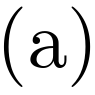
\includegraphics{figures/(a).png}

}

}

\end{minipage}%
%
\begin{minipage}[t]{0.01\linewidth}

{\centering 

~

}

\end{minipage}%
%
\begin{minipage}[t]{0.45\linewidth}

{\centering 

\raisebox{-\height}{

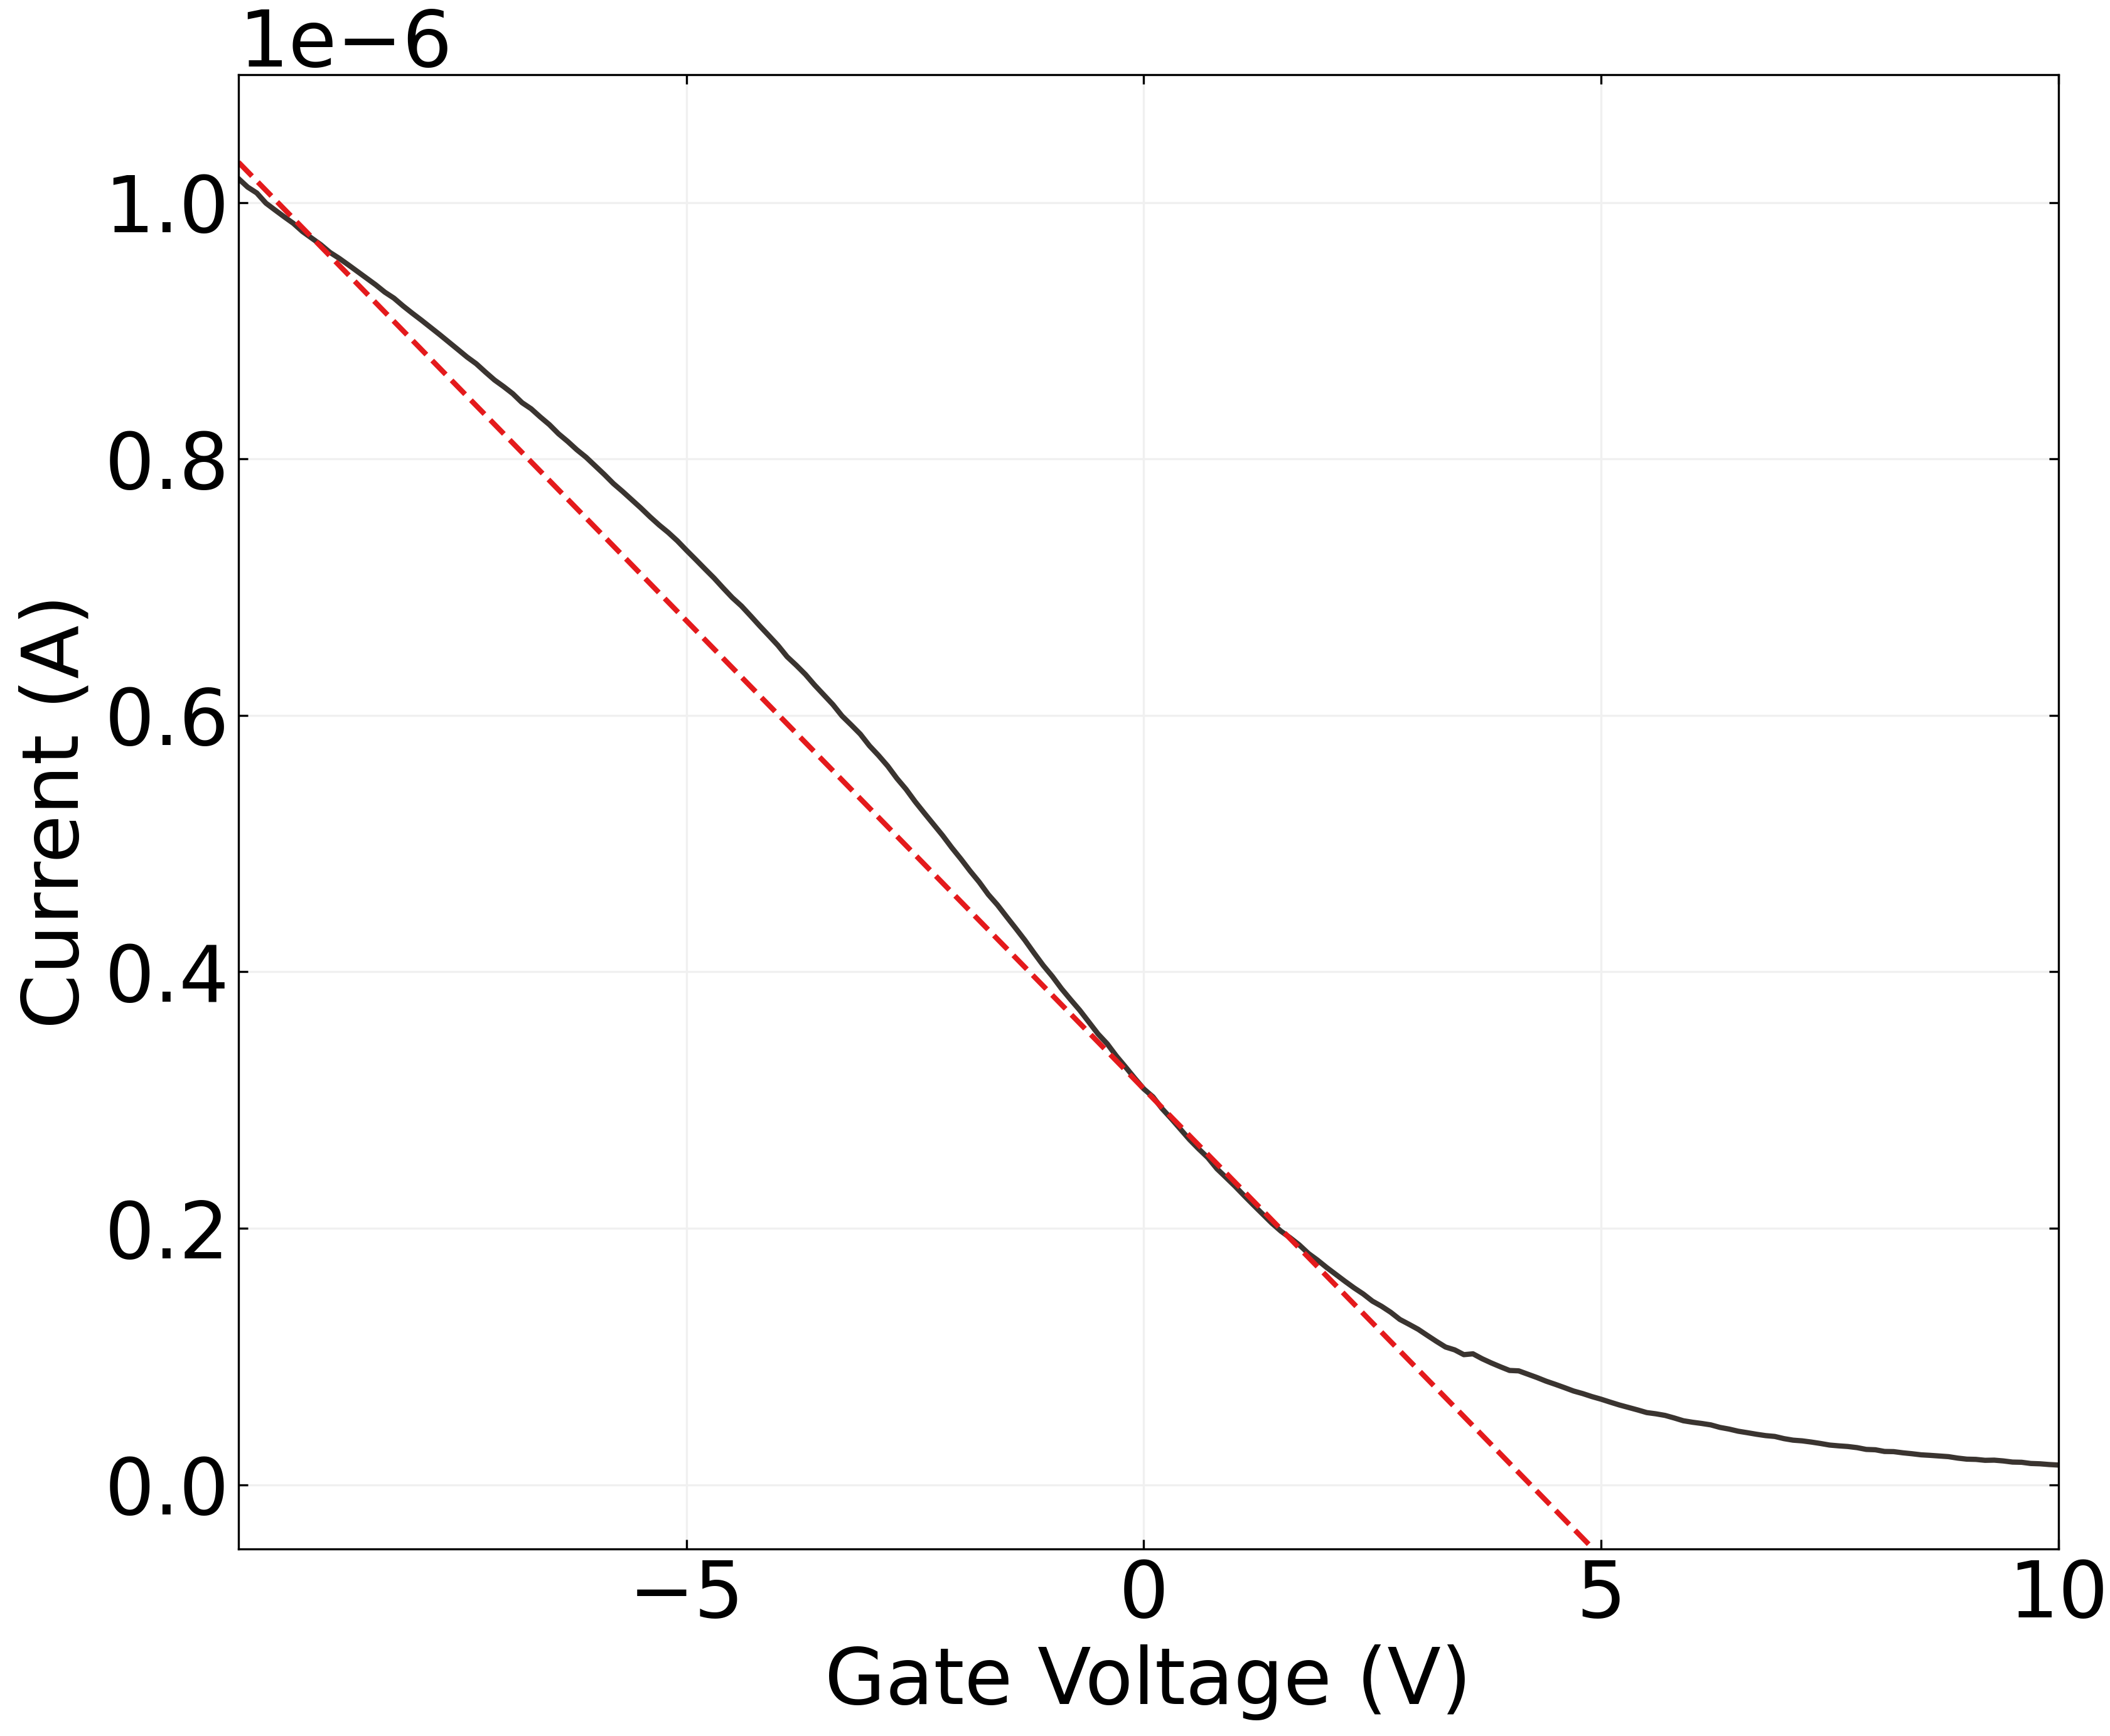
\includegraphics{figures/ch2/Q5C10ch5transconductance.png}

}

}

\end{minipage}%
%
\begin{minipage}[t]{0.01\linewidth}

{\centering 

~

}

\end{minipage}%
%
\begin{minipage}[t]{0.03\linewidth}

{\centering 

\raisebox{-\height}{

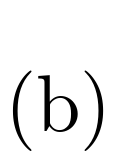
\includegraphics{figures/(b).png}

}

}

\end{minipage}%
%
\begin{minipage}[t]{0.01\linewidth}

{\centering 

~

}

\end{minipage}%
%
\begin{minipage}[t]{0.45\linewidth}

{\centering 

\raisebox{-\height}{

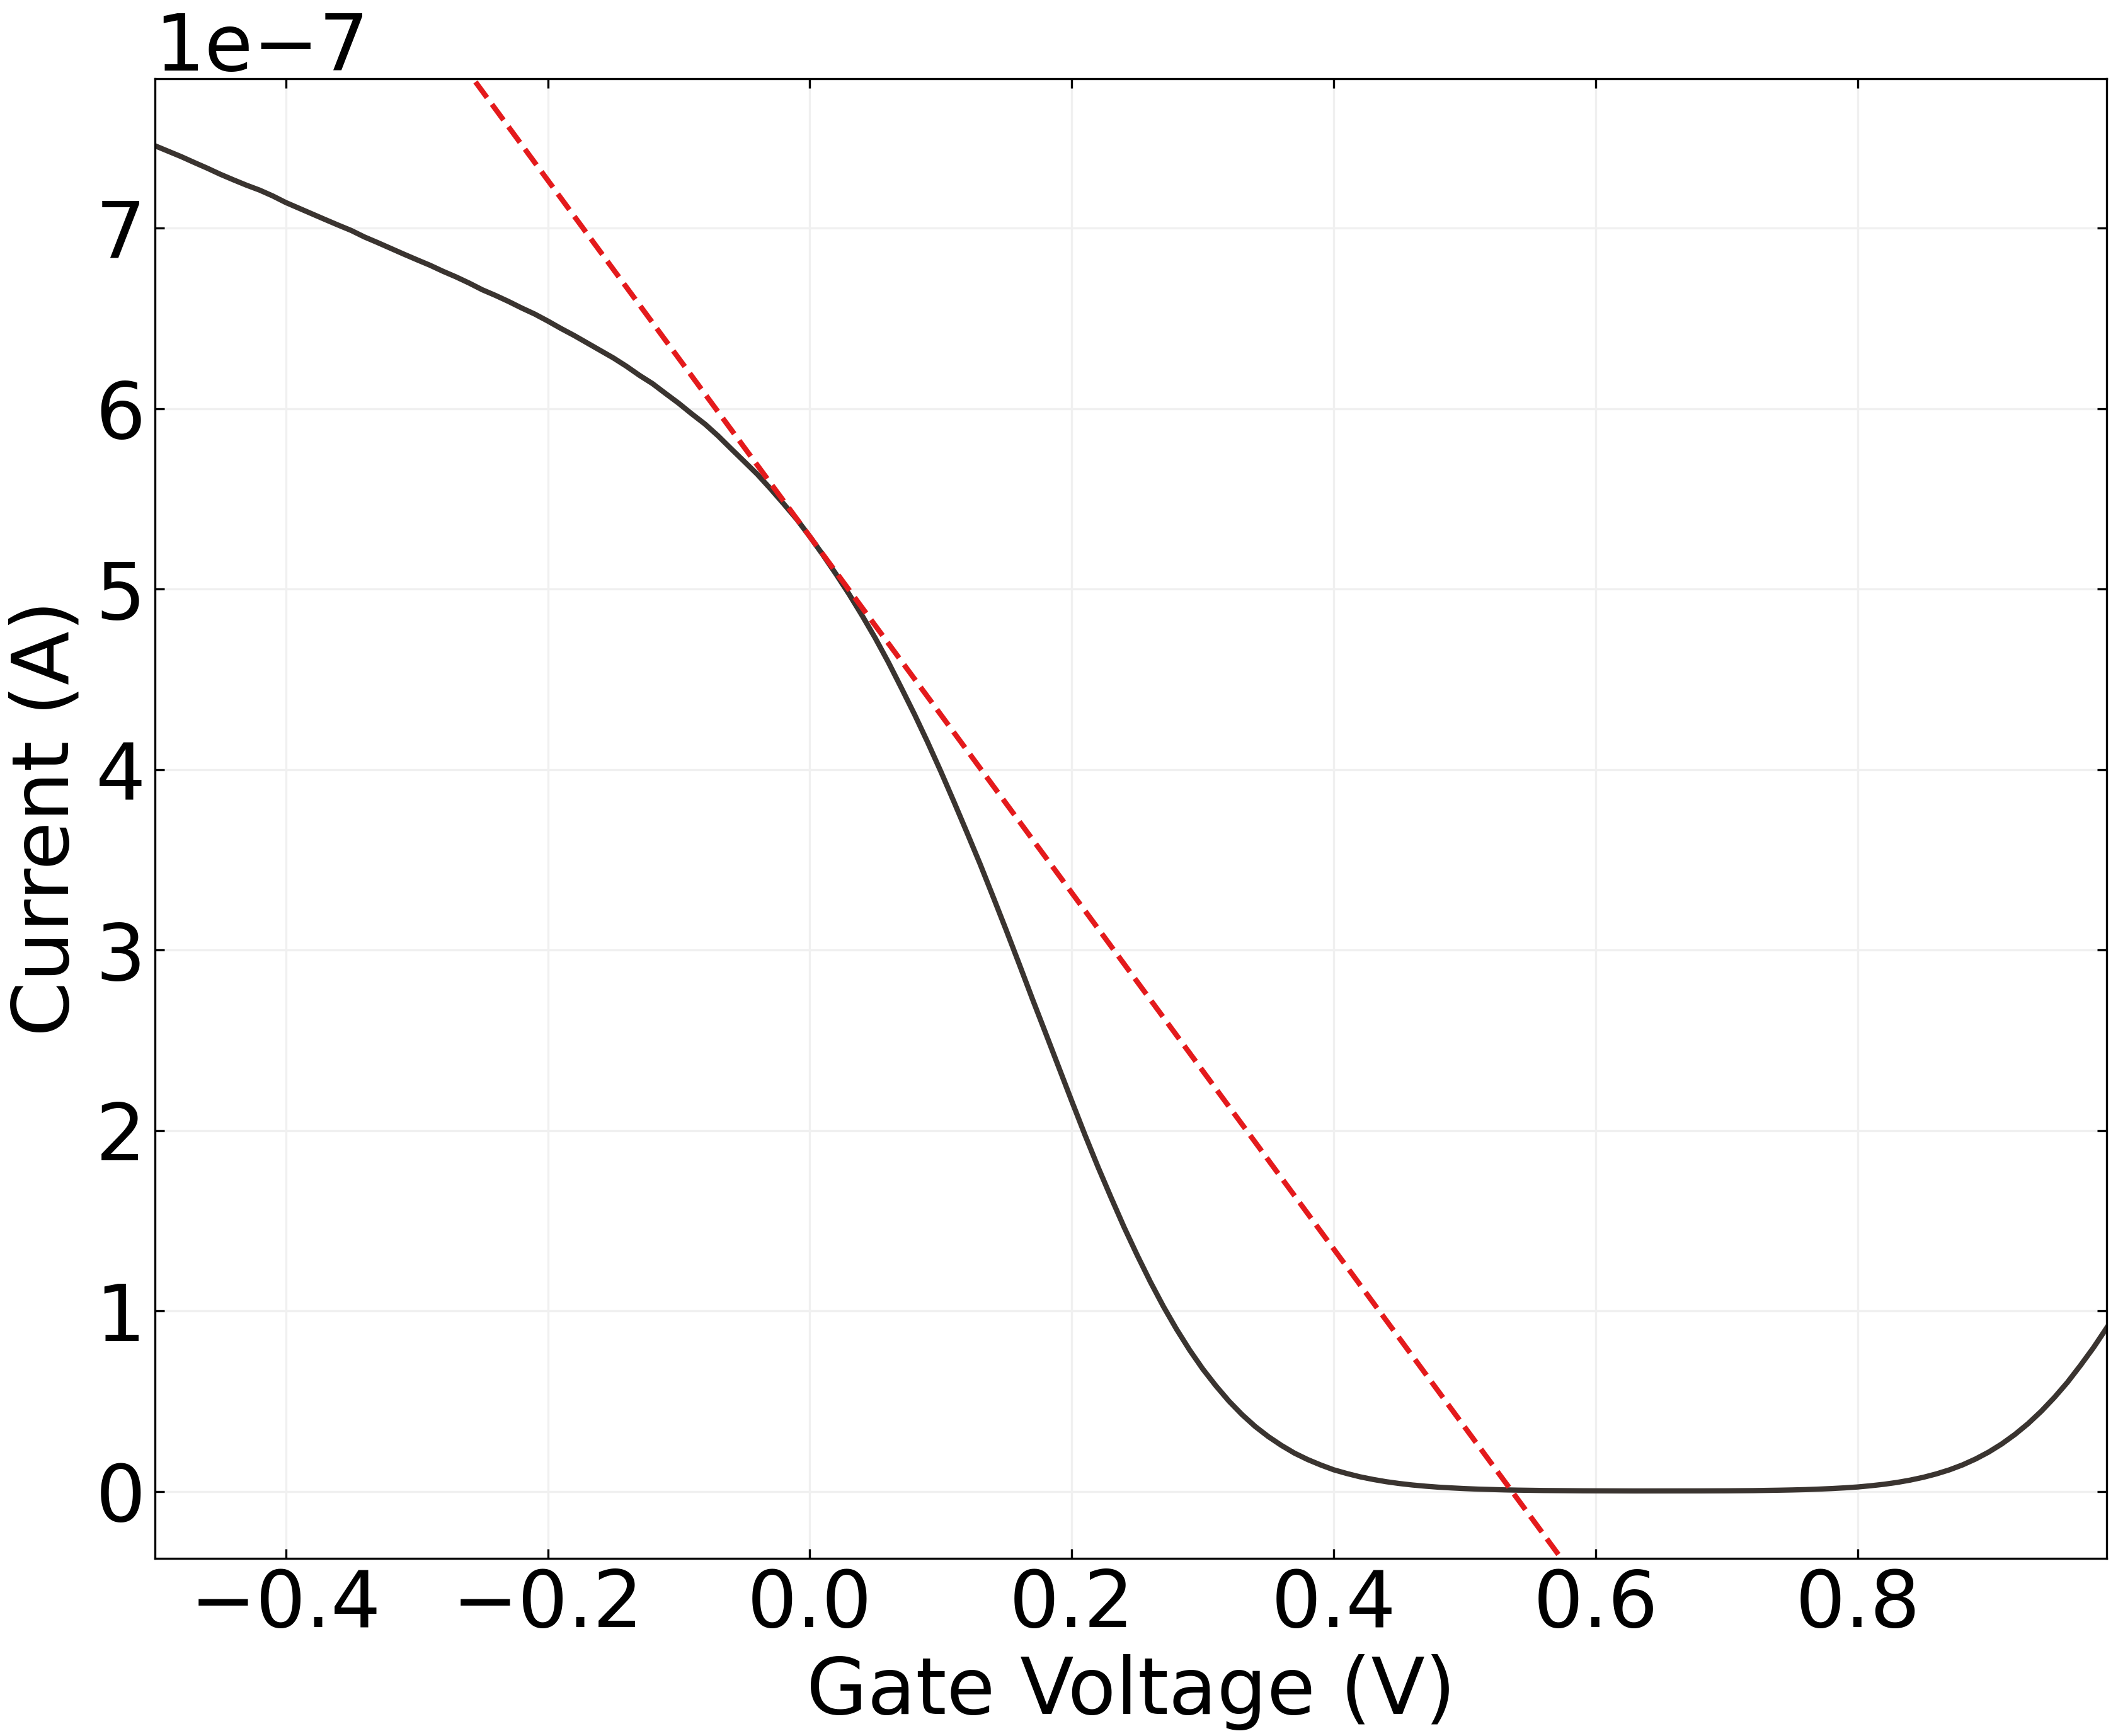
\includegraphics{figures/ch2/NTQ31C5ch1transconductance.png}

}

}

\end{minipage}%
%
\begin{minipage}[t]{0.01\linewidth}

{\centering 

~

}

\end{minipage}%
\newline
\begin{minipage}[t]{0.03\linewidth}

{\centering 

\raisebox{-\height}{

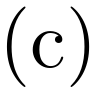
\includegraphics{figures/(c).png}

}

}

\end{minipage}%
%
\begin{minipage}[t]{0.01\linewidth}

{\centering 

~

}

\end{minipage}%
%
\begin{minipage}[t]{0.45\linewidth}

{\centering 

\raisebox{-\height}{

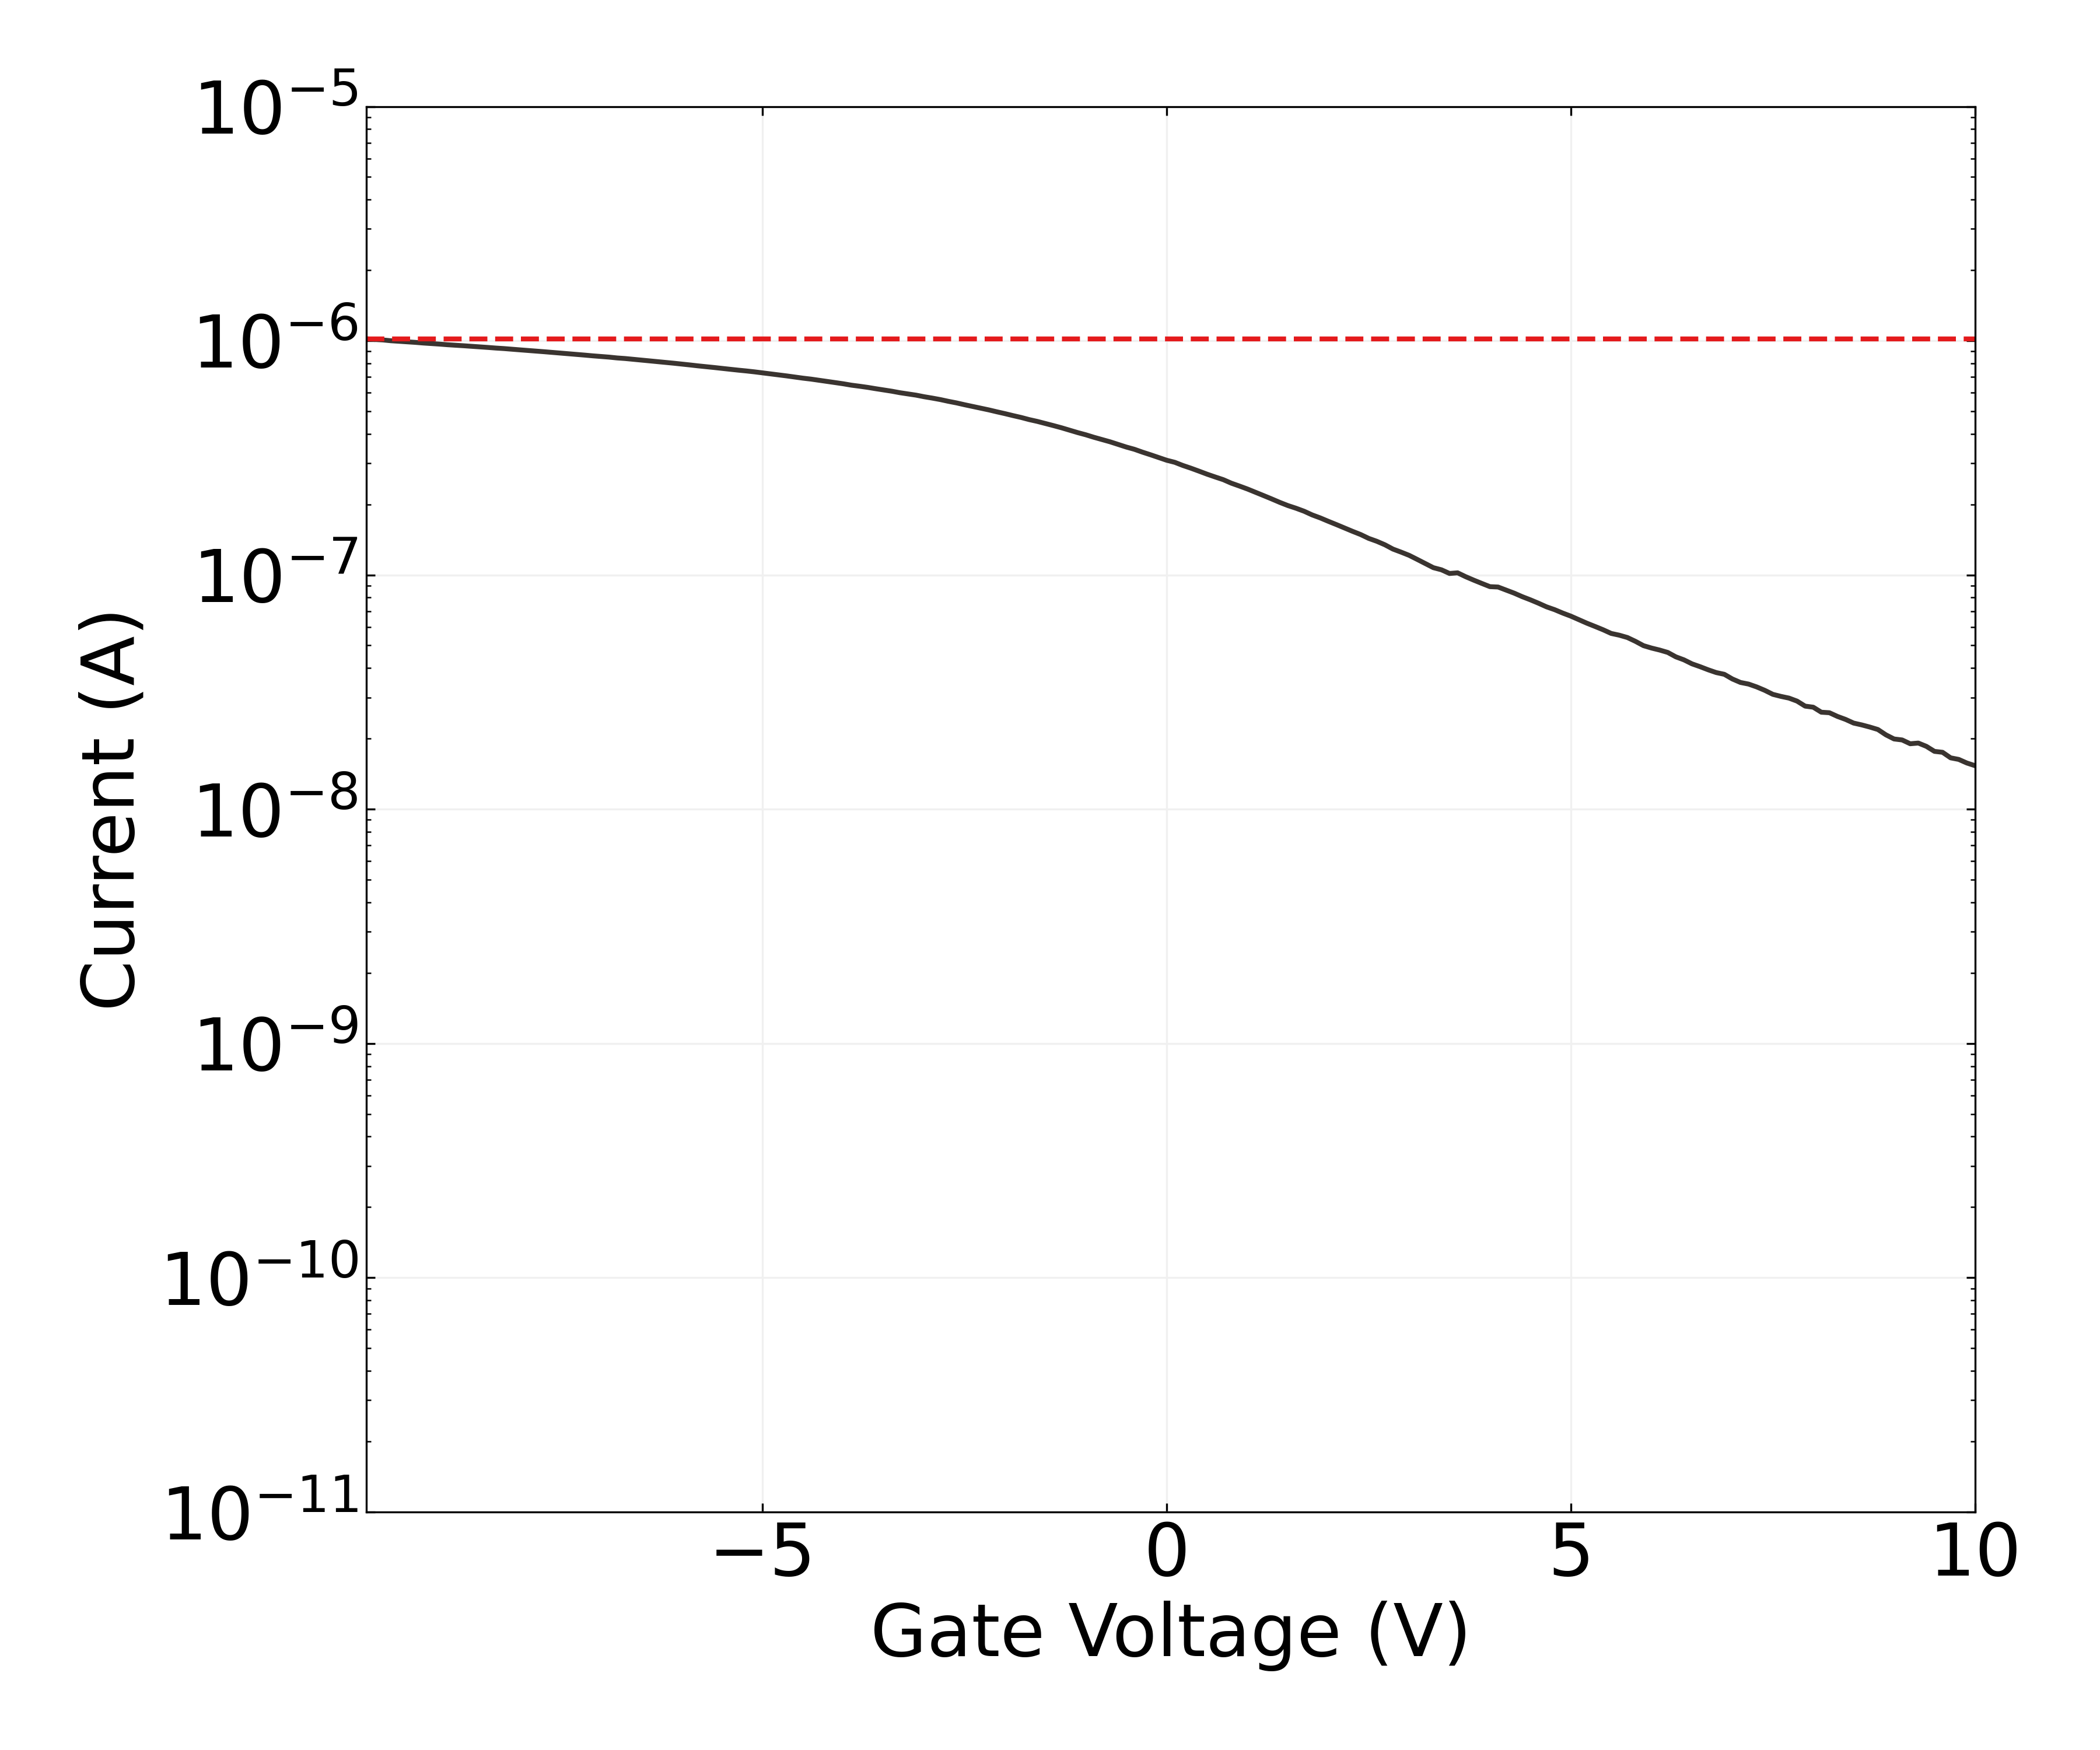
\includegraphics{figures/ch2/Q5C10ch5on_current.png}

}

}

\end{minipage}%
%
\begin{minipage}[t]{0.01\linewidth}

{\centering 

~

}

\end{minipage}%
%
\begin{minipage}[t]{0.03\linewidth}

{\centering 

\raisebox{-\height}{

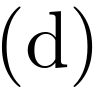
\includegraphics{figures/(d).png}

}

}

\end{minipage}%
%
\begin{minipage}[t]{0.01\linewidth}

{\centering 

~

}

\end{minipage}%
%
\begin{minipage}[t]{0.45\linewidth}

{\centering 

\raisebox{-\height}{

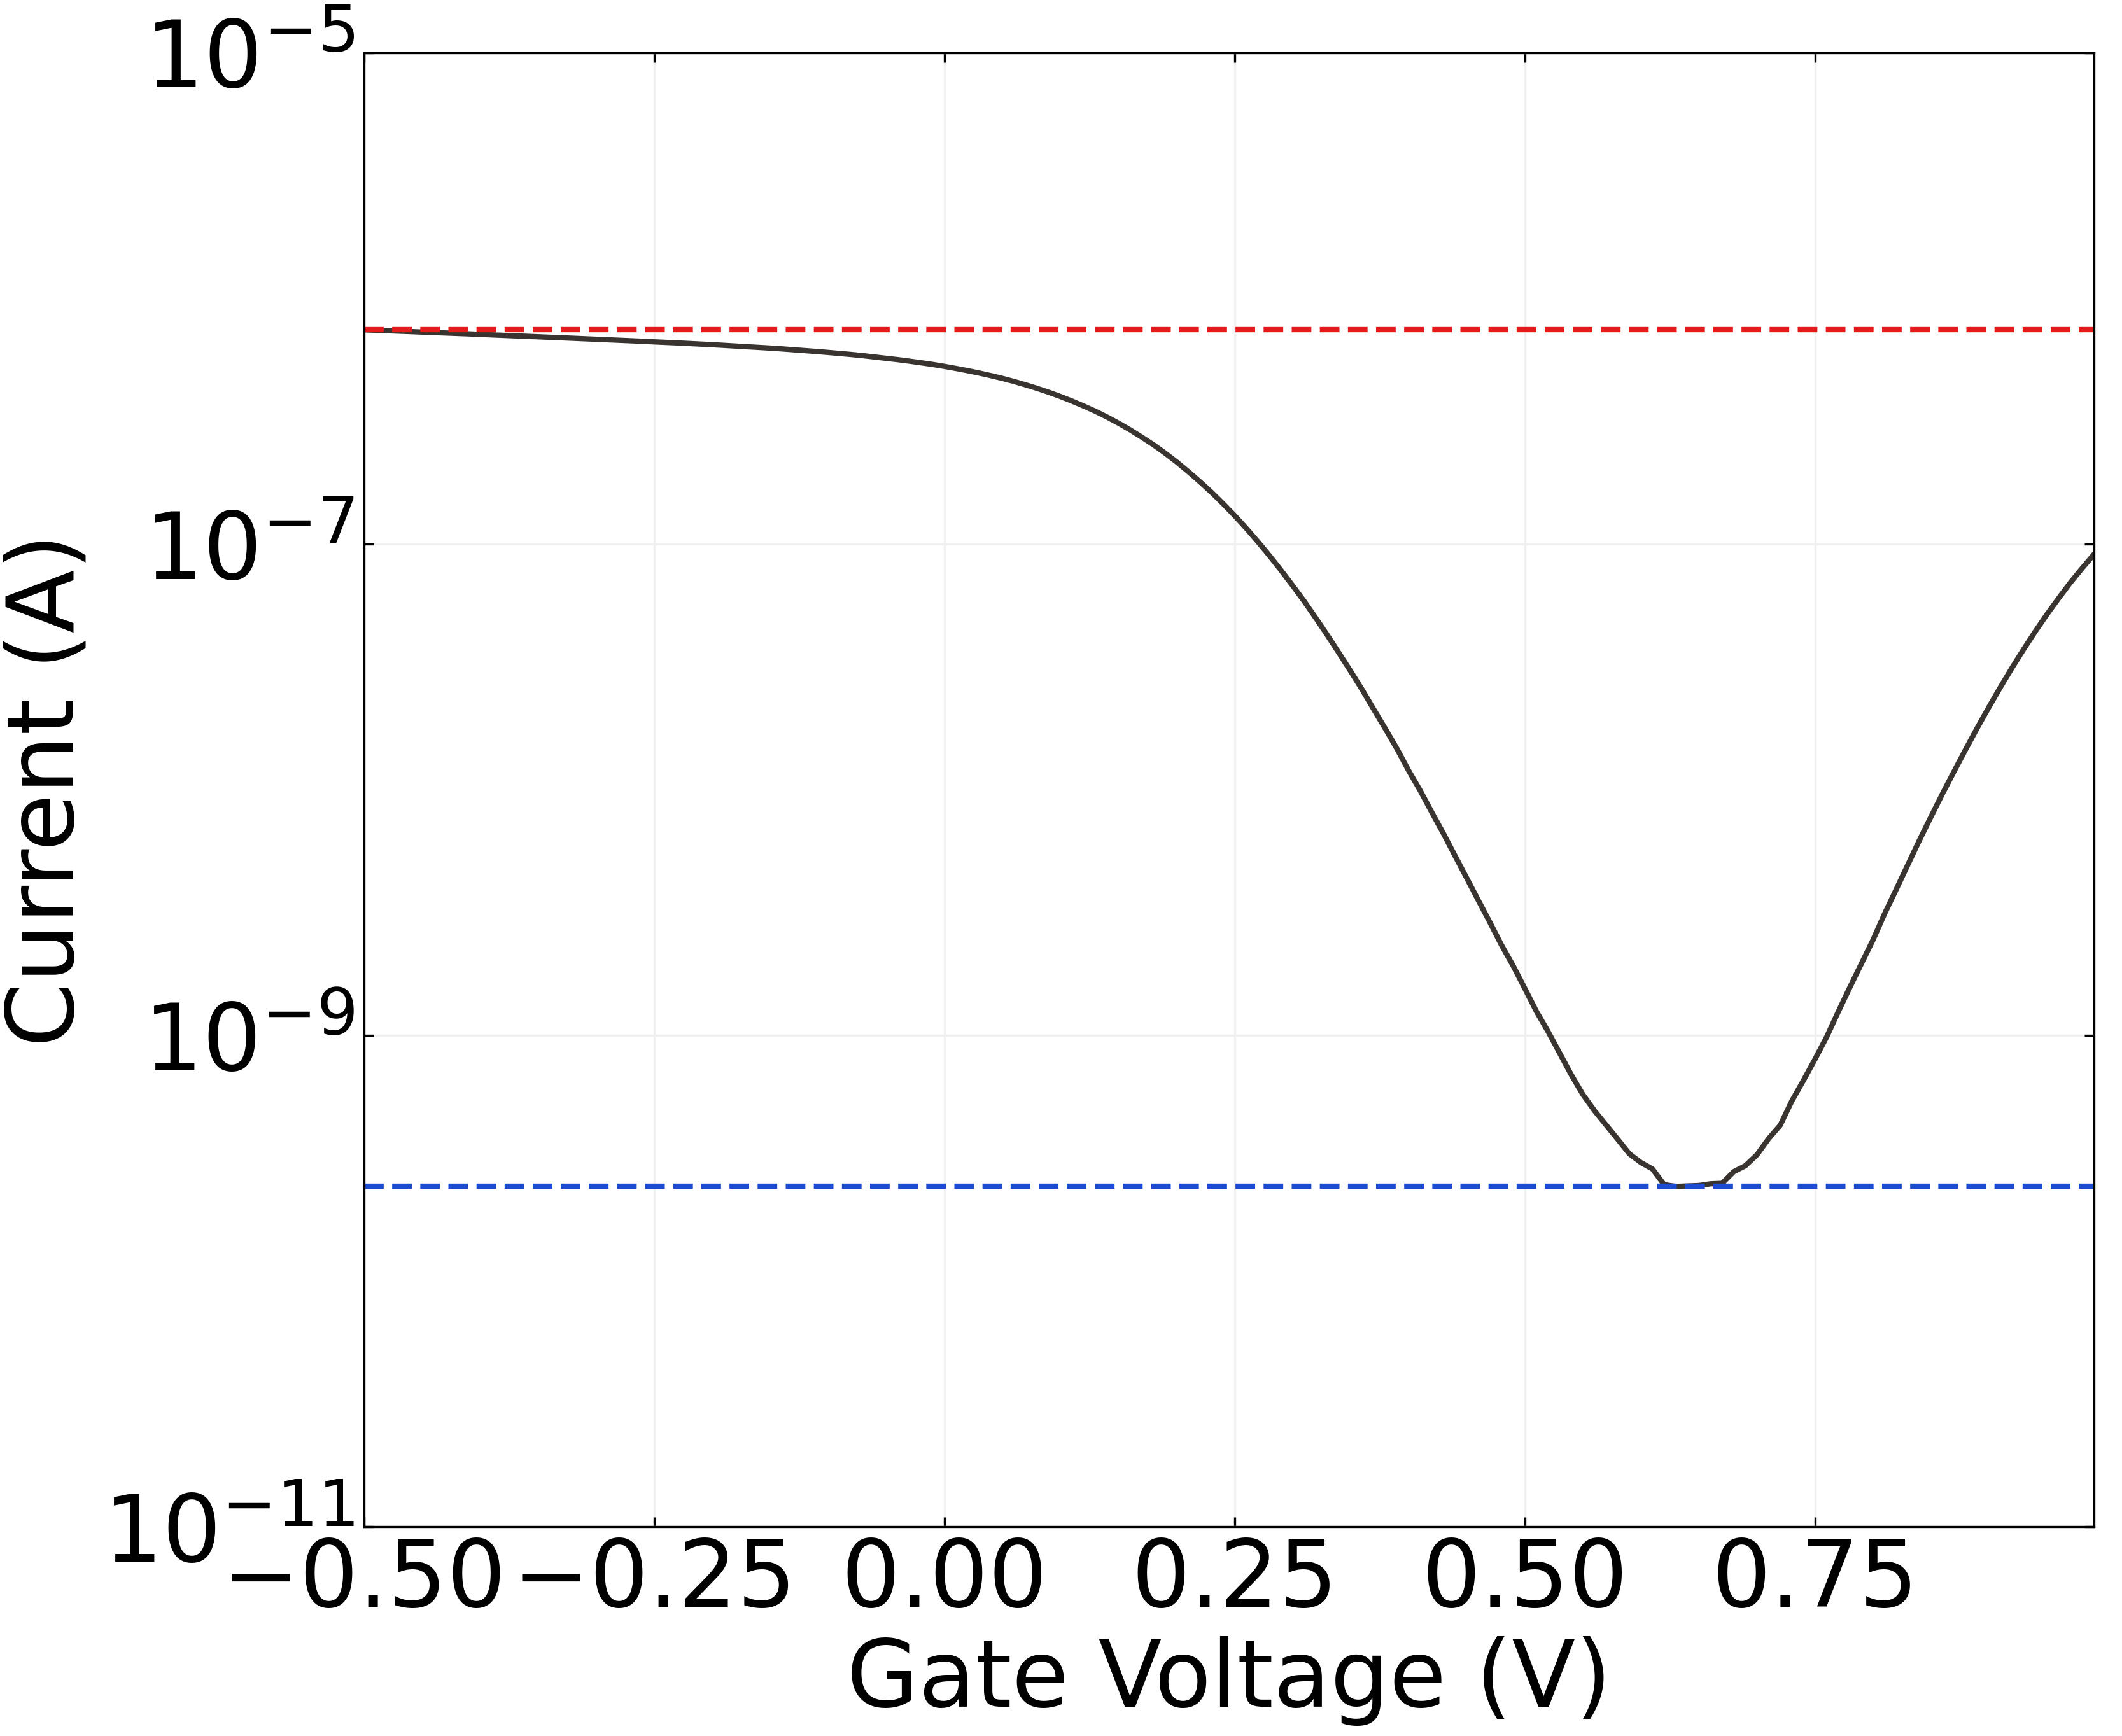
\includegraphics{figures/ch2/NTQ31C5ch1on_off_current.png}

}

}

\end{minipage}%
%
\begin{minipage}[t]{0.01\linewidth}

{\centering 

~

}

\end{minipage}%

\caption{\label{fig-gating-transfer}Examples of field-effect transistor
transfer characteristics taken at \(V_{ds}\) = 100 mV from two different
device channels. A linear scale is used in (a) and (b), while a
logarithmic scale is used in (c) and (d). The device channel in (a) and
(c) was backgated while the device channel in (b) and (d) was
liquid-gated. The linear fit with gradient corresponding to
transconductance at \(V_g\) = 0 V is shown in (a) and (b) with a dotted
red line. The ``on'' current in (c) and (d) is shown with a red
horizontal line, while the ``off'' current in (d) is shown with a blue
horizontal line.}

\end{figure}

Channel carriers in a FET can be accelerated by a sufficiently high
gate-channel field into surmounting the insulating barrier between the
gate and channel. This is known as `breakdown'. The breakdown voltage
\(V_b\) gives an upper limit to the bias able to be applied across the
device without the device being destroyed. Percolation theory can be
used to explain breakdown. As energetic carriers pass through the oxide,
defects are created randomly. When these random defects are dense enough
to form a chain from the gate to the semiconductor, a short is created
and breakdown occurs. With decreased oxide thickness the the required
voltage for breakdown also decreases, due to increased carrier
tunnelling.

\begin{itemize}
\tightlist
\item
  oxide layer leakages
\end{itemize}

Then leakage also occurs when electrolyte conducts

\hypertarget{current-sampling}{%
\subsection{Current Sampling}\label{current-sampling}}

It is important to account for the changes in current that occur during
a sensing run that are unrelated to sensing, and try to minimise these
changes as much as possible. These changes are due to a variety of
causes and can be categorised as various types of noise and baseline
drift. (1/f noise paper, heller paper)

\hypertarget{graphene-field-effect-transistors}{%
\section{Graphene Field-Effect
Transistors}\label{graphene-field-effect-transistors}}

\hypertarget{sec-electrical-characterisation-graphene}{%
\subsection{Electrical
Characterisation}\label{sec-electrical-characterisation-graphene}}

\begin{figure}

{\centering 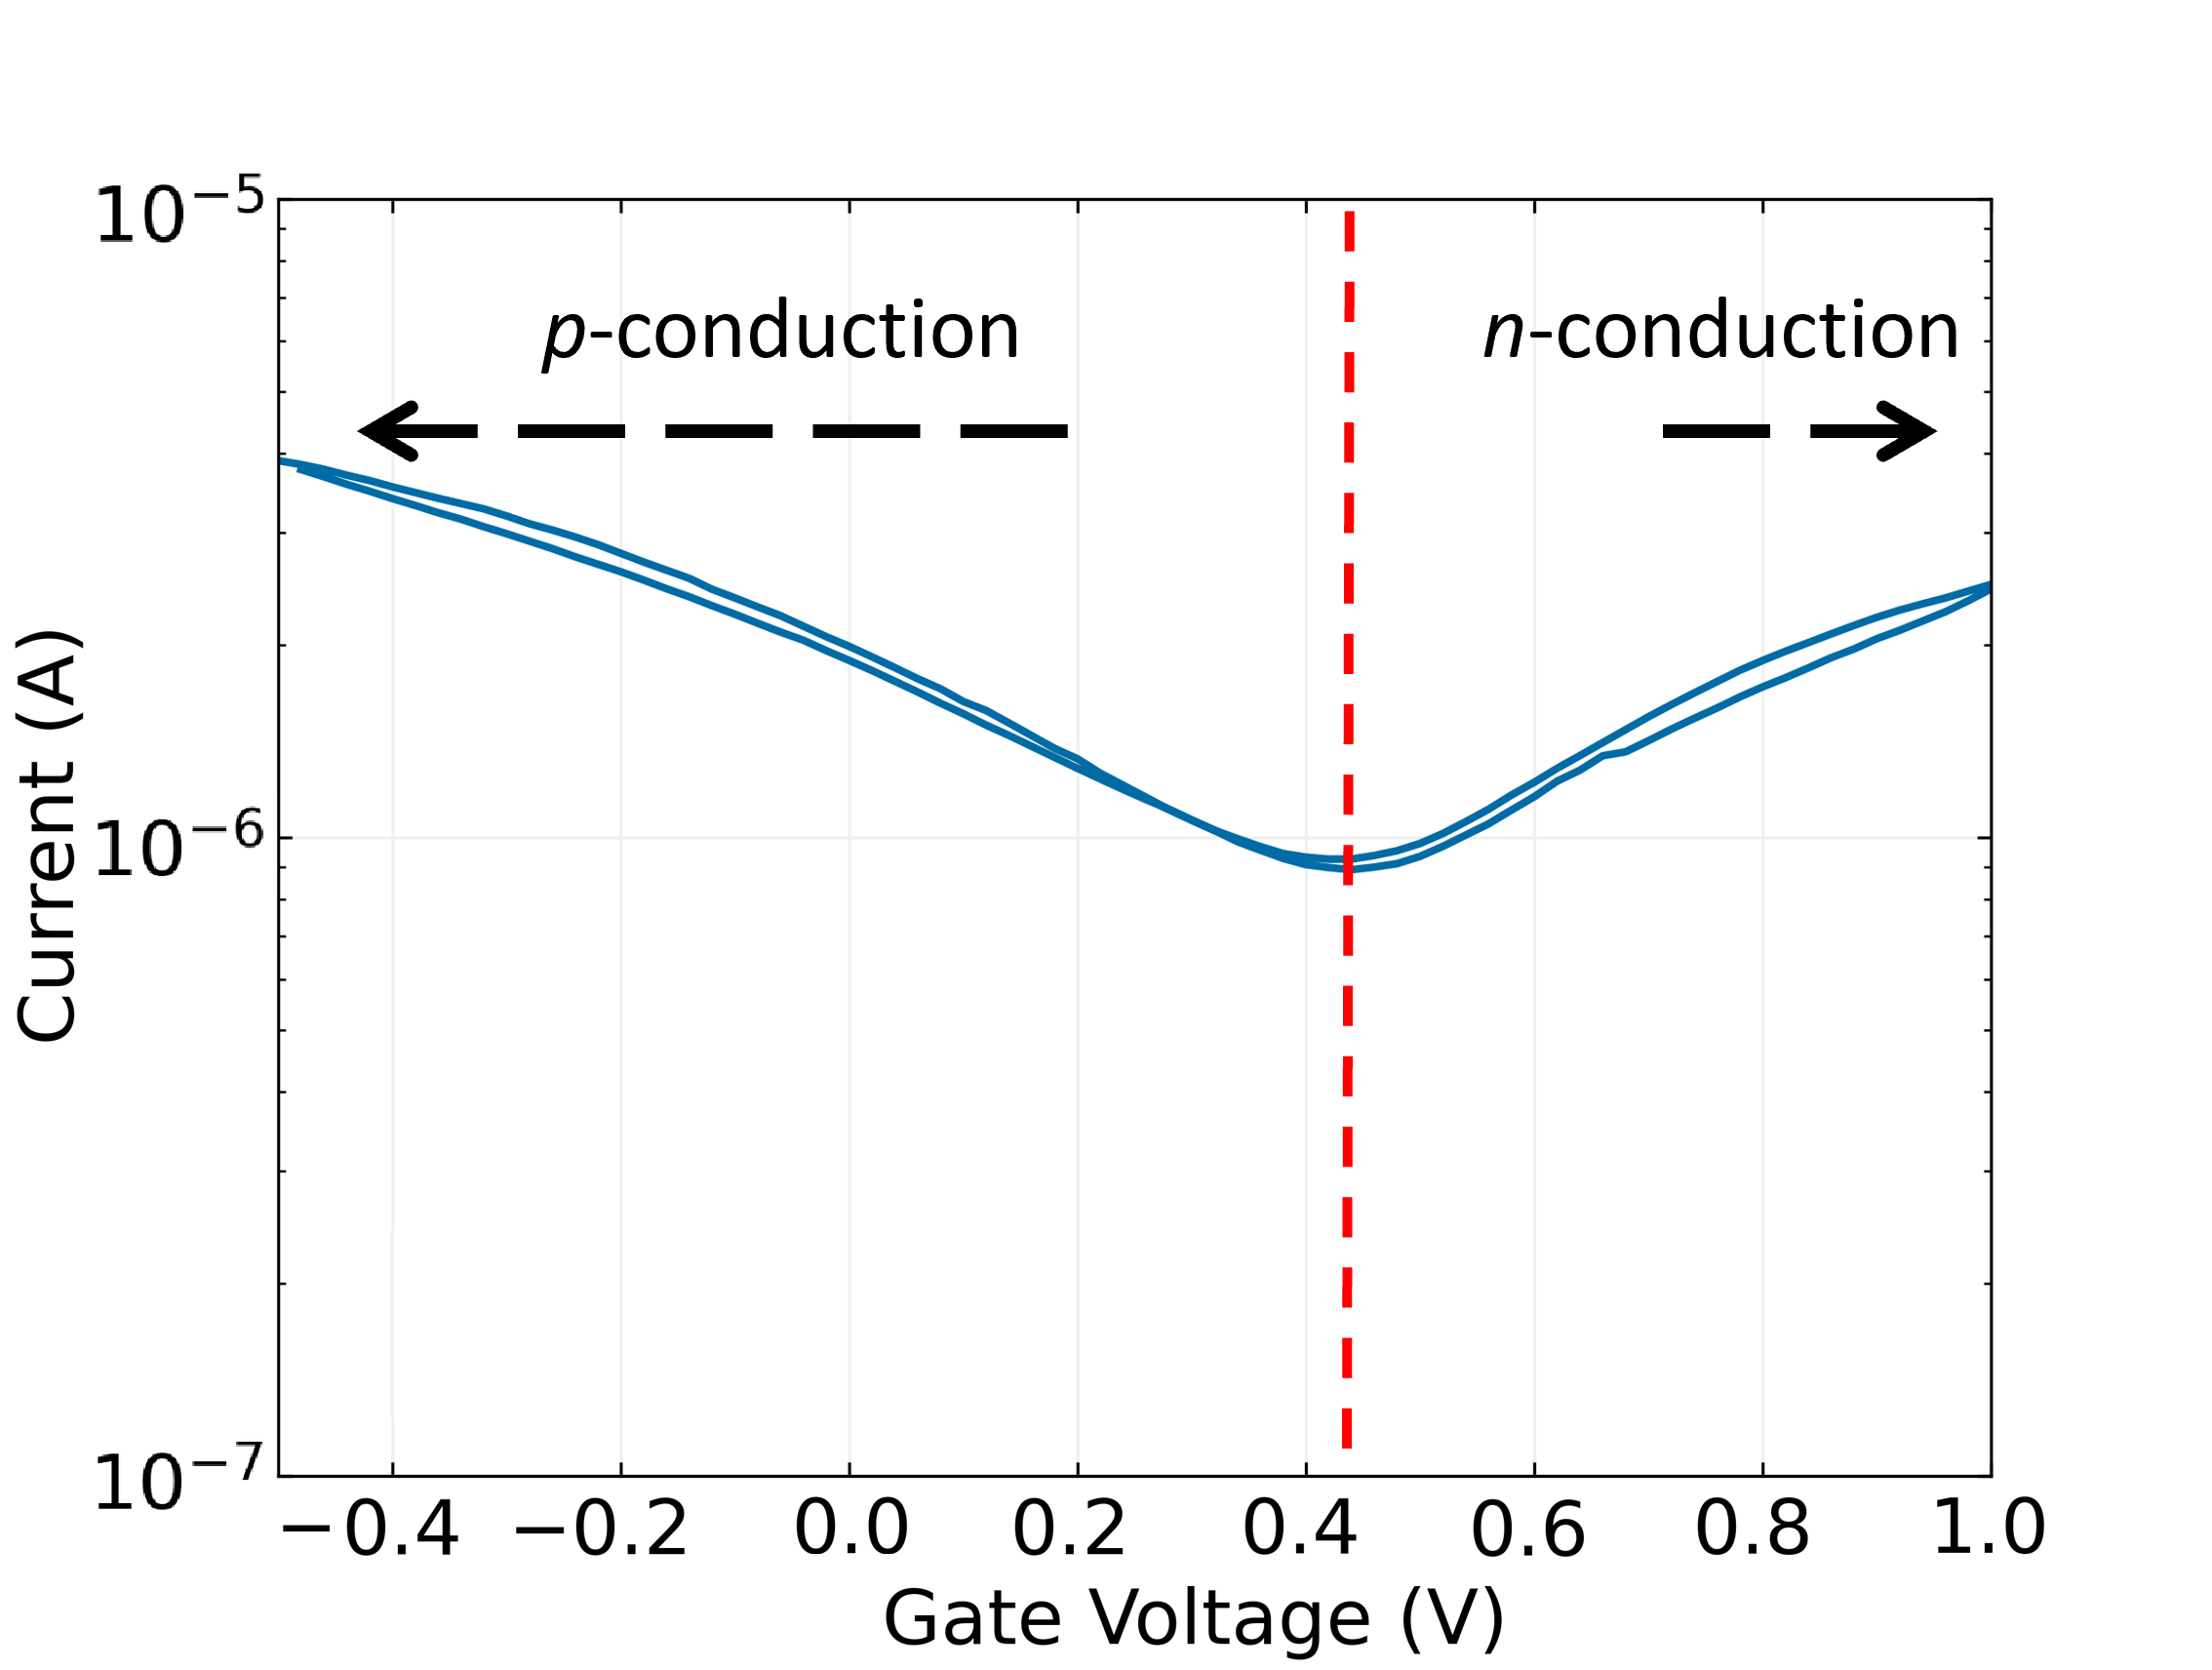
\includegraphics[width=0.6\textwidth,height=\textheight]{figures/ch2/Graphene_transfer.png}

}

\caption{\label{fig-linker-raman}Transfer characteristics of a graphene
field-effect transistor channel showing the regions of hole conduction
and electron conduction. The red dotted line indicates the Dirac point
voltage of the device channel.}

\end{figure}

As graphene field-effect transistors do not possess a characteristic
`off' regime. In normal operation of a GFET, the lowest voltage
obtainable by gating is known as the Dirac voltage
\autocite{Murugathas2020}.

Quantative measurement of leftward shift in transfer curve Use minima of
curve in reverse sweep direction (more consistent than reading in
forward sweep direction) I compared the transfer characteristics after
then rinse steps to the pristine characteristics Transfer shifts where
current drops to zero are excluded (indicates delamination/damage to
channel)

\hypertarget{random-network-carbon-nanotube-field-effect-transistors}{%
\section{Random-Network Carbon Nanotube Field-Effect
Transistors}\label{random-network-carbon-nanotube-field-effect-transistors}}

\hypertarget{composition-and-chirality}{%
\subsection{Composition and Chirality}\label{composition-and-chirality}}

A single-walled carbon nanotube (SWCNT) consists of a graphene sheet, a
flat carbon lattice with hexagonal cells, rolled up into a cylinder.
Since their discovery in 1991, a wide range of device applications for
carbon nanotubes (CNTs) have been proposed, based on CNTs being highly
sensitive to their environment \autocite{Iijima1991,Dekker1999}. This
high sensitivity is due to the high surface-to-volume ratio of the CNTs,
which maximises the exposure of this electrically sensitive structure to
its surroundings \autocite{Yao2021,Shkodra2021}. SWCNT-based devices
consume little power, operate quickly and are highly flexible
\autocite{Shkodra2021}. Nanotubes in a network can have semiconducting
characteristics (s-CNTs) or metallic characteristics (m-CNTs), depending
on their chirality \autocite{Martel1998,Kong2000}. A single CNT will
therefore have different properties than a network of CNTs, where the
individual electrical properties of the CNT tubes are averaged out
across the network \autocite{Battie2010}. The contact between the
electrodes and carbon nanotubes determines the behaviour of channel
carriers. The properties of electrodes generally used in CNT FETs means
they usually operate as \(p\)-type transistors \autocite{Yao2021}.

Able to conduct ballistically, good coupling between gate and channel
electric fields with carbon nanotube devices which enables shorter
channel sizes \autocite{Avouris2007} carbon nanotube devices in the
electrolyte-gated layout have stronger channel-gate coupling than the
back-gated layout \autocite{Heller2009a}

Semiconducting carbon nanotubes have particular advantages for use in
sensor applications, including a high carrier mobility, compatibility
with many biological targets, and ease of processing
\autocite{Shkodra2021}.

\hypertarget{carbon-nanotube-networks}{%
\subsection{Carbon Nanotube Networks}\label{carbon-nanotube-networks}}

Schottky barriers form between the metallic and semiconducting carbon
nanotubes within a network

\hypertarget{sec-electrical-characterisation-CNT}{%
\subsection{Electrical
Characterisation}\label{sec-electrical-characterisation-CNT}}

\begin{figure}

\begin{minipage}[t]{0.03\linewidth}

{\centering 

\raisebox{-\height}{

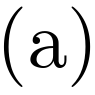
\includegraphics{figures/(a).png}

}

}

\end{minipage}%
%
\begin{minipage}[t]{0.01\linewidth}

{\centering 

~

}

\end{minipage}%
%
\begin{minipage}[t]{0.45\linewidth}

{\centering 

\raisebox{-\height}{

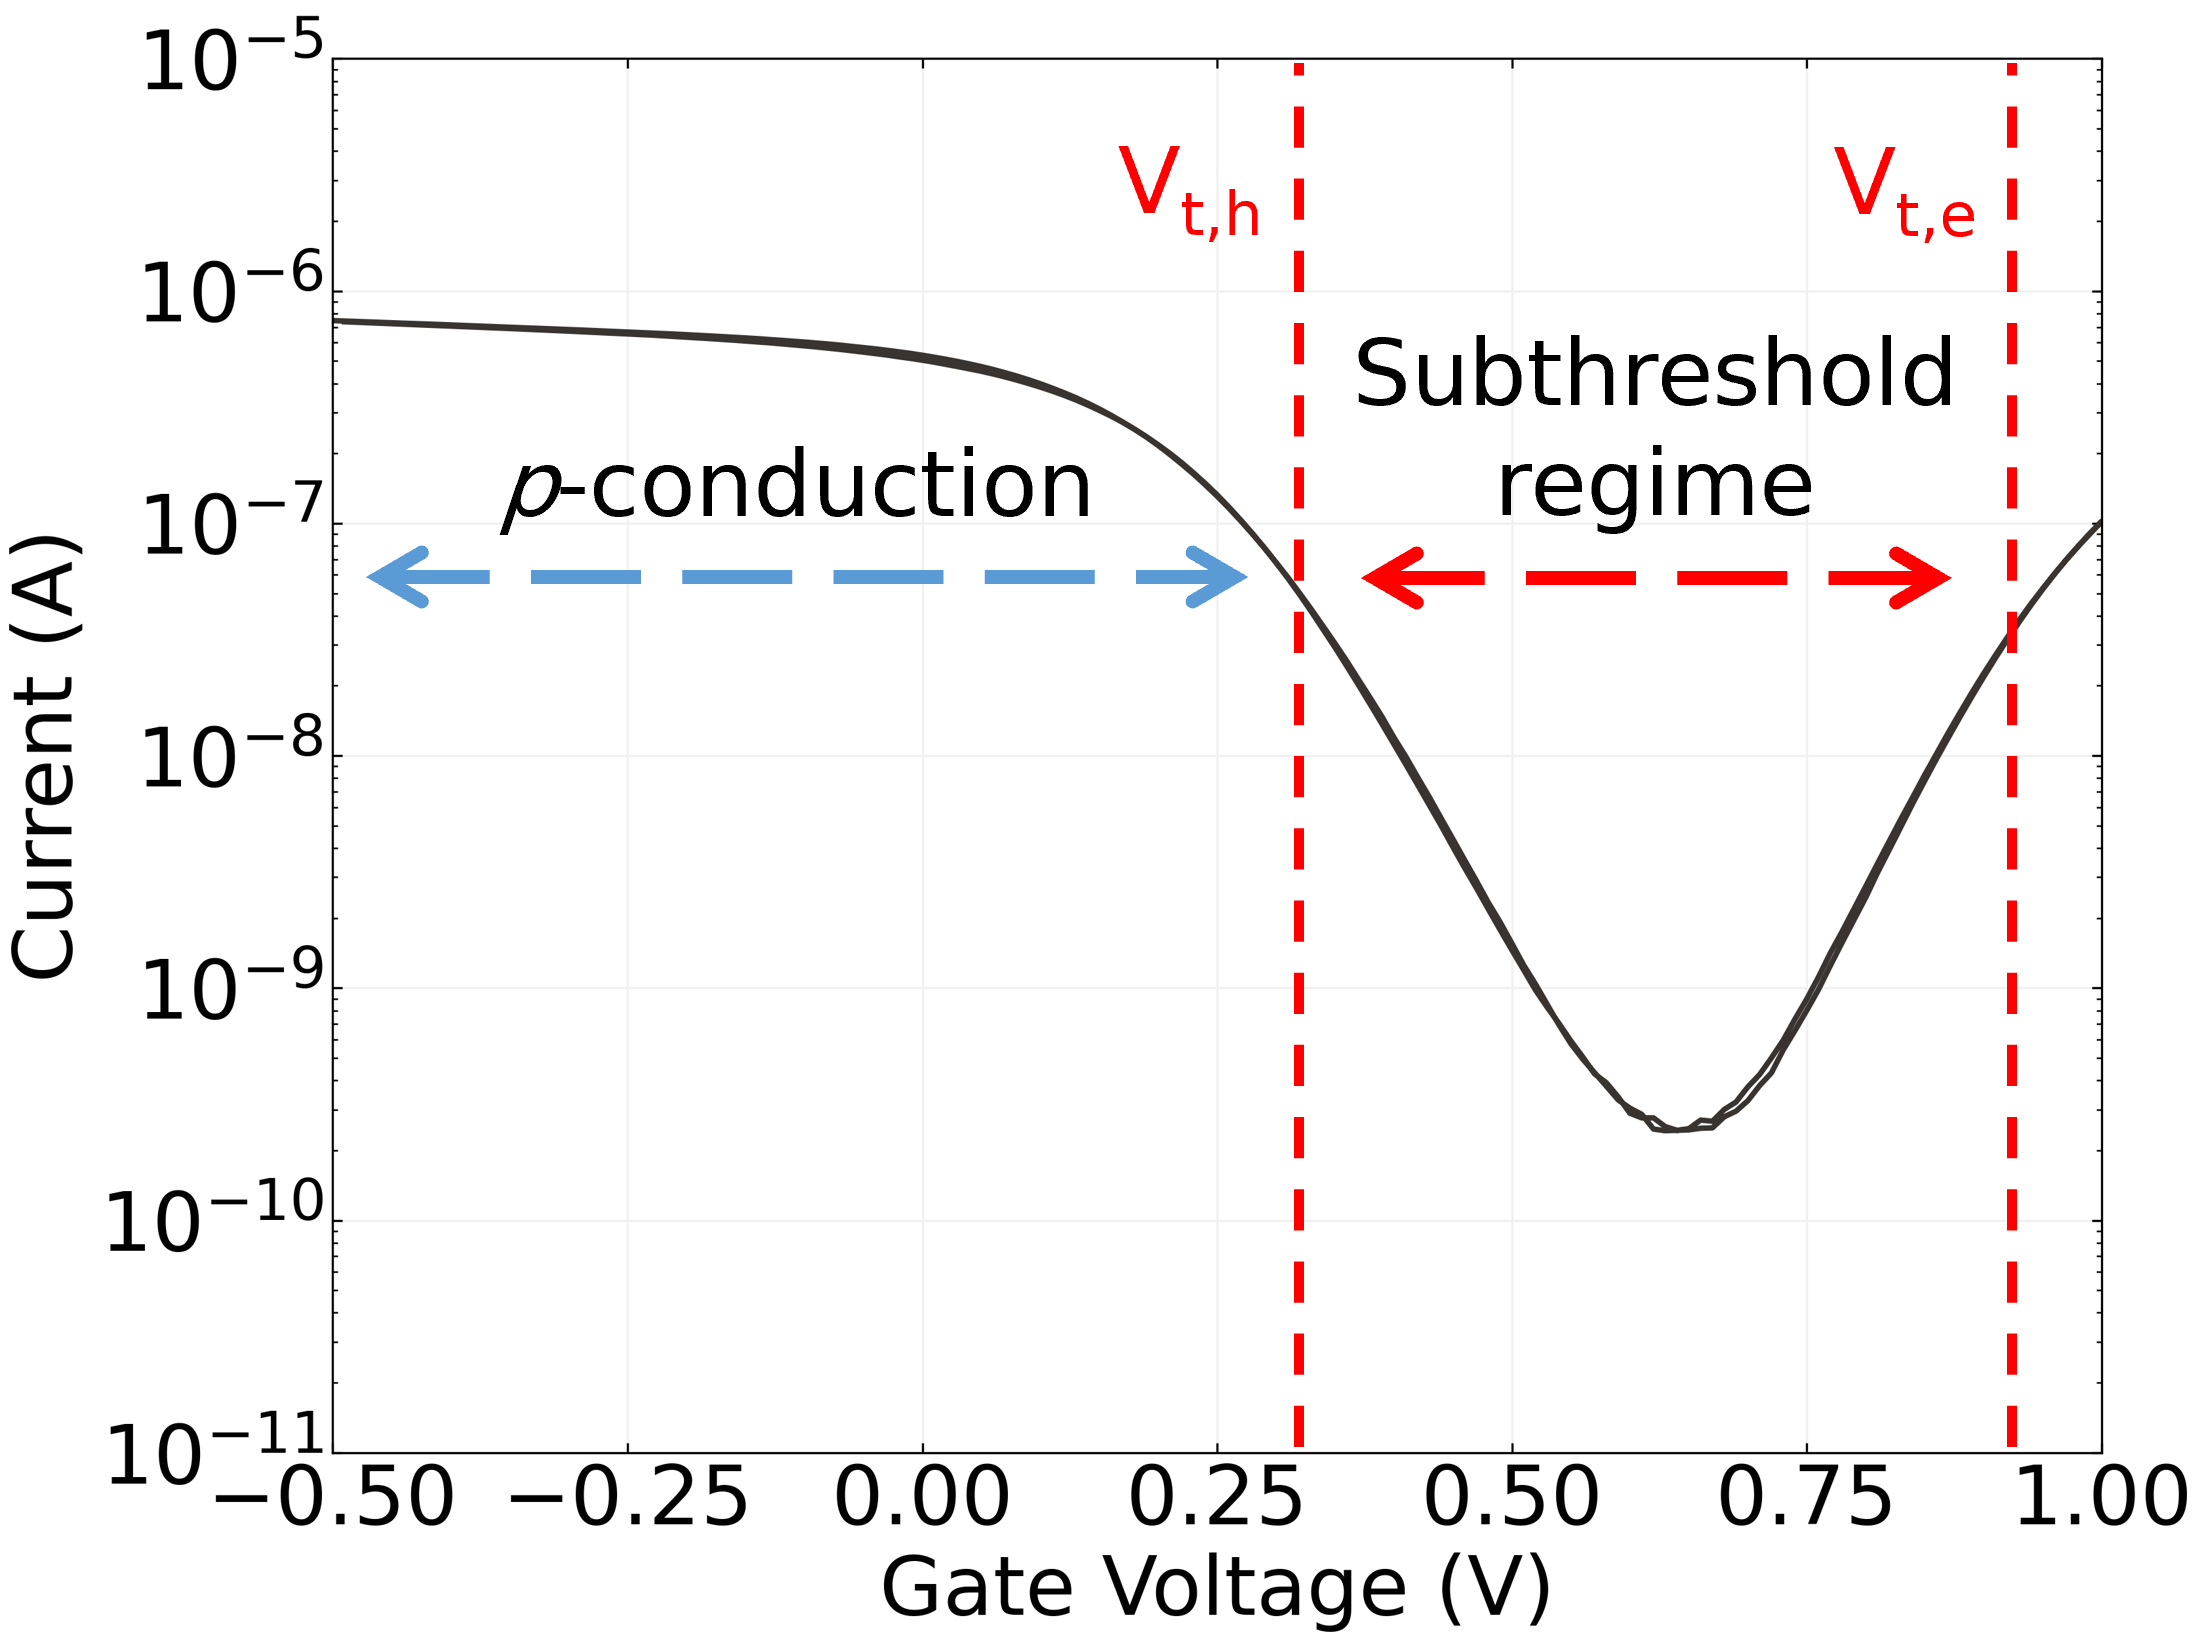
\includegraphics{figures/ch2/CNT_transfer_1.png}

}

}

\end{minipage}%
%
\begin{minipage}[t]{0.01\linewidth}

{\centering 

~

}

\end{minipage}%
%
\begin{minipage}[t]{0.03\linewidth}

{\centering 

\raisebox{-\height}{

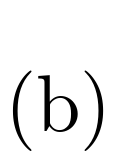
\includegraphics{figures/(b).png}

}

}

\end{minipage}%
%
\begin{minipage}[t]{0.01\linewidth}

{\centering 

~

}

\end{minipage}%
%
\begin{minipage}[t]{0.45\linewidth}

{\centering 

\raisebox{-\height}{

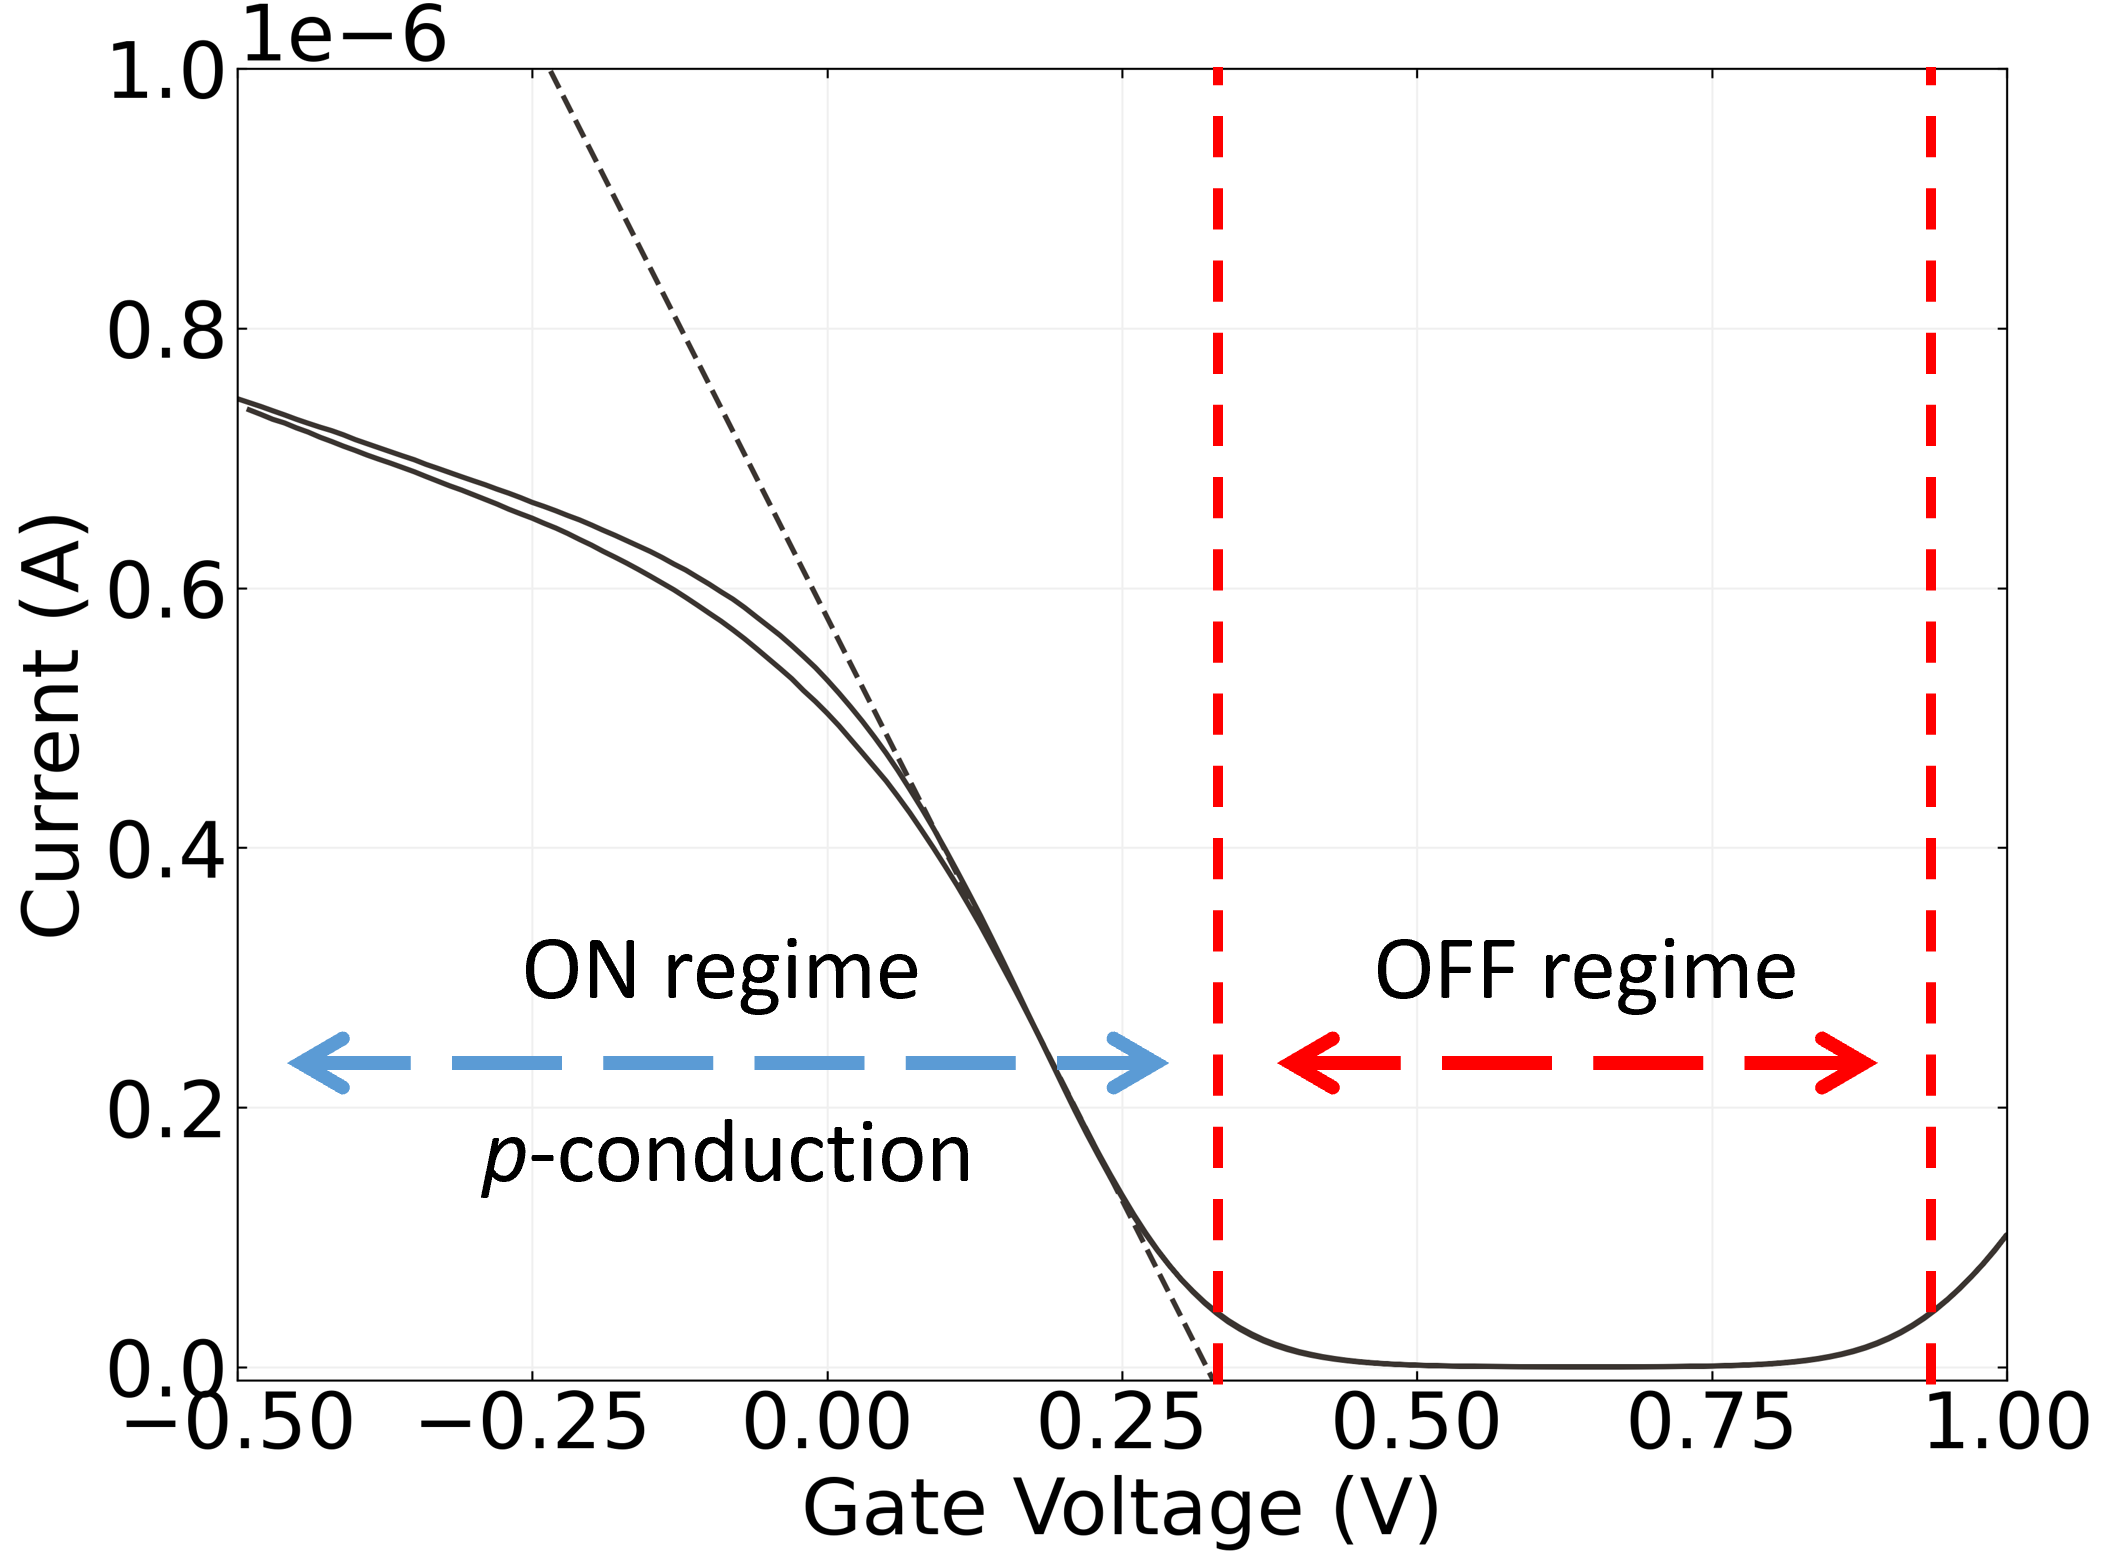
\includegraphics{figures/ch2/CNT_transfer_2.png}

}

}

\end{minipage}%
%
\begin{minipage}[t]{0.01\linewidth}

{\centering 

~

}

\end{minipage}%

\caption{\label{fig-literature-characteristics}Transfer characteristics
of a single carbon nanotube network field-effect transistor channel,
using a logarithmic scale in (a) and using a linear scale in (b) to
emphasise different features of the same dataset. The subthreshold slope
is shown with a black dotted line, while the threshold voltages are
shown with red dotted lines. The ON and OFF regimes are also indicated
on both figures.}

\end{figure}

Like graphene transistors, carbon nanotube transistors are naturally
ambipolar: they can conduct both electrons and holes. Holes travel at
highly negative voltages, while electrons travel at highly positive
voltages. At intermediary voltages, both electrons and holes flow.
Carbon nanotube transistors can also be doped into behaving as a
unipolar transistor \autocite{Avouris2007}. If heavily oxygen doped, the
semiconducting carbon nanotubes will exhibit \(p\)-type behaviour, with
current flow only occuring in a negative bias state
\autocite{Shkodra2021}.

\hypertarget{threshold-voltage}{%
\subsubsection*{Threshold Voltage}\label{threshold-voltage}}
\addcontentsline{toc}{subsubsection}{Threshold Voltage}

The threshold voltage is the voltage required to fully deplete the
device channel of charge carriers \autocite{Martel1998}. It can be
estimated by extrapolating the linear part of the transfer
characteristics of a device to the \(V_g\) axis.

The FET turns on at the `threshold voltage', \(V_g\) = \(V_t\). For the
\(p\)-type FET, when \(V_g\) \textgreater{} \(V_t\), \(I_d\) increases
linearly.

After decreasing past \(V_t\), \(I_d\) stays constant at its `on' value
\(I_{ON}\). The ratio of \(I_{ON}\) to the \(I_{OFF}\) current is known
as the FET device's `on-off ratio', \(I_{ON}/I_{OFF}\). The threshold
voltage can be calculated by using an FET's transfer characteristics.
From extrapolating the trendline of the linear region to the \(V_g\)
axis, the intercept \(V_{gInt}\) is approximately equivalent to \(V_t\)
\autocite{Sze2006}.

Threshold Voltage: minimum gate-to-source voltage that is needed to
create a conducting path between the electrodes

Quantative measurement of leftward shift in transfer curve Use minima of
curve in reverse sweep direction (more consistent than reading in
forward sweep direction) I compared the transfer characteristics after
then rinse steps to the pristine characteristics Transfer shifts where
current drops to zero are excluded (indicates delamination/damage to
channel)

Second quantative measurement of leftward shift in transfer curve Use
curve in reverse sweep direction (more consistent than reading in
forward sweep direction) Separate readings for left and right hand sides
of transfer curve (left side = electrons dominant carrier, right side =
holes dominant carrier) Transfer shifts where current drops to zero are
excluded (indicates delamination/damage to channel) This gives us a
quantitative idea of whether the transfer shifts in slides 5/6 are
stable (remain the same/similar after rinse steps)

\cleardoublepage
\phantomsection
\addcontentsline{toc}{part}{Appendices}
\appendix

\hypertarget{sec-vapour-sensor-components}{%
\chapter{Vapour System Hardware}\label{sec-vapour-sensor-components}}

\hypertarget{tbl-vapour-sensor-components}{}
\begin{longtable}[t]{>{\raggedright\arraybackslash}p{5.5cm}>{\raggedright\arraybackslash}p{4.5cm}>{\raggedright\arraybackslash}p{3.75cm}}
\caption{\label{tbl-vapour-sensor-components}Major components used in construction of the vapour delivery system
described in this thesis. }\tabularnewline

\toprule
Description & Part No. & Manufacturer\\
\midrule
Mass flow controller, 20 sccm full scale & GE50A013201SBV020 & MKS Instruments\\
Mass flow controller, 200 sccm full scale & GE50A013202SBV020 & MKS Instruments\\
Mass flow controller, 500 sccm full scale & FC-2901V & Tylan\\
Analogue flowmeter, 240 sccm max. flow & 116261-30 & Dwyer\\
Micro diaphragm pump & P200-B3C5V-35000 & Xavitech\\
\addlinespace
Analogue flow controller, for micro diaphragm pump & X3000450 & Xavitech\\
10 mL Schott bottle & 218010802 & Duran\\
PTFE connection cap system & Z742273 & Duran\\
Baseline VOC-TRAQ flow cell, red & 043-951 & Mocon\\
Humidity and temperature sensor & T9602 & Telaire\\
\addlinespace
Enclosure, for humidity and temperature sensor & MC001189 & Multicomp Pro\\
\bottomrule
\end{longtable}

\hypertarget{sec-python}{%
\chapter{Python Code for Data Analysis}\label{sec-python}}

\hypertarget{code-repository}{%
\section{Code Repository}\label{code-repository}}

The code used for general analysis of field-effect transistor devices in
this thesis was written with Python 3.8.8. Contributors to the code used
include Erica Cassie, Erica Happe, Marissa Dierkes and Leo Browning. The
code is located on GitHub and the research group OneDrive, and is
available on request.

\hypertarget{sec-histogram-analysis}{%
\section{Atomic Force Microscope Histogram
Analysis}\label{sec-histogram-analysis}}

The purpose of this code is to analyse atomic force microscope (AFM)
images of carbon nanotube networks in .xyz format taken using an atomic
force microscope and processed in Gwyddion (see
\textbf{?@sec-afm-characterisation}). It was originally designed by
Erica Happe in Matlab, and adapted by Marissa Dierkes and myself for use
in Python. The code imports the .xyz data and sorts it into bins 0.15 nm
in size for processing. To perform skew-normal distribution fits, both
\emph{scipy.optimize.curve\_fit} and \emph{scipy.stats.skewnorm} modules
are used in this code.

\hypertarget{sec-raman-analysis}{%
\section{Raman Spectroscopy Analysis}\label{sec-raman-analysis}}

The purpose of this code is to analyse a series of Raman spectra taken
at different points on a single film (see
\textbf{?@sec-raman-characterisation}). Data is imported in a series of
tab-delimited text files, with the low wavenumber spectrum (100
cm\(^{-1} - 650\) cm\(^{-1}\)) and high wavenumber spectrum (1300
cm\(^{-1} - 1650\) cm\(^{-1}\)) imported in separate datafiles for each
scan location.

\hypertarget{sec-field-effect-transistor-analysis}{%
\section{Field-Effect Transistor
Analysis}\label{sec-field-effect-transistor-analysis}}

The purpose of this code is to analyse electrical measurements taken of
field-effect transistor (FET) devices. Electrical measurements were
either taken from the Keysight 4156C Semiconductor Parameter Analyser,
National Instruments NI-PXIe or Keysight B1500A Semiconductor Device
Analyser as discussed in \textbf{?@sec-electrical-characterisation}; the
code is able to analyse data in .csv format taken from all three
measurement setups. The main Python file in the code base consists of
three related but independent modules: the first analyses and plots
sensing data from the FET devices, the second analyses and plots
transfer characteristics from channels across a device, and the third
compares individual channel characteristics before and after a
modification or after each of several modifications. The code base also
features a separate config file and style sheet which govern the
behaviour of the main code. The code base was designed collaboratively
by myself and Erica Cassie over GitHub using the Sourcetree Git GUI.


\backmatter
\printbibliography


\end{document}
